%%%%%%%%%%%%%%%%%%%%%%%%%%%%%%%%%%%%%%%%%%%%%%%%%%%%%%%%%%%%%%%%%%%%
%% I, the copyright holder of this work, release this of into the
%% public domain. This applies worldwide. In some countries this may
%% not be legally possible; if so: I grant anyone the right to use
%% this work for any purpose, without any conditions, unless such
%% conditions are required by law.
%%%%%%%%%%%%%%%%%%%%%%%%%%%%%%%%%%%%%%%%%%%%%%%%%%%%%%%%%%%%%%%%%%%%

\documentclass[
    %twoside,   % Printed version
    %printed,   % Printed version
    digital,    % PC version
    oneside,    % PC version
    color,
    11pt,
    nocover,
    notable,
    nolof,
    nolot,
    final
  %% More options are listed in the user guide at
  %% <http://mirrors.ctan.org/macros/latex/contrib/fithesis/guide/mu/fi.pdf>.
]{fithesis3}
%% The following section sets up the locales used in the thesis.
\usepackage[resetfonts]{cmap} %% We need to load the a T2A font encoding
%\usepackage[utf8]{inputenc}
\usepackage[T1]{fontenc}  % T2a commented %% to use the Cyrillic fonts with Russian texts.
\usepackage[
  main=english, %% By using `czech` or `slovak` as the main locale
                %% instead of `english`, you can typeset the thesis
                %% in either Czech or Slovak, respectively.
  english %german, russian, slovak %% The additional keys allow
]{babel}        %% foreign texts to be typeset as follows:
%%
%%   \begin{otherlanguage}{german}  ... \end{otherlanguage}
%%   \begin{otherlanguage}{russian} ... \end{otherlanguage}
%%   \begin{otherlanguage}{czech}   ... \end{otherlanguage}
%%   \begin{otherlanguage}{slovak}  ... \end{otherlanguage}
%%
%% For non-Latin scripts, it may be necessary to load additional
%% fonts:
%\usepackage{paratype}
%\def\textrussian#1{{\usefont{T2A}{PTSerif-TLF}{m}{rm}#1}}

%%
%% The following section sets up the metadata of the thesis.
\thesissetup{
    date          = \the\year/\the\month/\the\day,
    university    = mu,
    faculty       = fi,
    type          = mgr,
    author        = Michal Hajas,
    gender        = m,
    advisor       = {RNDr. Petr Švenda, Ph.D.},
    title         = {Analysis of pseudo-random number generators based on lightweight cryptographic primitives},
    TeXtitle      = {Analysis of pseudo-random number generators based on lightweight cryptographic primitives},
    keywords      = {randomness testing, cryptanalysis, block functions, lightweight cryptography, pseudo-radnom number generators},
    TeXkeywords   = {randomness testing, cryptanalysis, block functions, lightweight cryptography, pseudo-radnom number generators},
}


\thesislong{abstract}{%
This thesis proposes a process of randomness analysis using a CryptoStreams tool which provides a unified interface for cryptographic primitives for generating sequences within a configurable environment. The process is illustrated on analysis of distinguishability of output from a pseudo-random number generators. Generators are analyzed in four different testing scenarios. In each scenario tested generators were provided a different type of input with some lousy properties (e.g. low Hamming weight). For analysis of randomness of sequences, four different software tools were used. Three well-known statistical batteries: NIST STS, Dieharder and TestU01, and principally simple, yet powerful, tool BoolTest developed at Faculty of Informatics, Masaryk University. Results are presenting the ability of tested generators to provide an output which is indistinguishable from random data and also a comparison of the success of used software tools to distinguish analyzed sequences.
}

\thesislong{thanks}{%
I would like to thank everybody who supported me during whole my studies. Especially to my supervisor RNDr. Petr Švenda, Ph.D. who was willing to help me with any issue, I fell into while working on this thesis.


\vspace*{17cm}\noindent{}\hspace*{-0.1cm}
Computational resources were supplied by the Ministry of Education, Youth and Sports of the Czech Republic under the Projects CESNET (Project No. LM2015042) and CERIT-Scientific Cloud (Project No. LM2015085) provided within the program Projects of Large Research, Development and Innovations Infrastructures.
}

%% The following section sets up the bibliography.
\usepackage{csquotes}
\usepackage[              %% When typesetting the bibliography, the
  backend=biber,          %% `numeric` style will be used for the
  style=numeric,          %% entries and the `numeric-comp` style
  citestyle=numeric-comp, %% for the references to the entries. The
  sorting=none,           %% entries will be sorted in cite order.
  sortlocale=auto         %% For more unformation about the available
]{biblatex}               %% `style`s and `citestyles`, see:
%% <http://mirrors.ctan.org/macros/latex/contrib/biblatex/doc/biblatex.pdf>.
\addbibresource{thesis.bib} %% The bibliograpic database within
                          %% the file `example.bib` will be used.
\usepackage{makeidx}      %% The `makeidx` package contains
\makeindex                %% helper commands for index typesetting.



%% These additional packages are used within the document:
\usepackage{paralist}
\usepackage{amsmath}
\usepackage{amsthm}
\usepackage{amsfonts}
\usepackage{url}

\usepackage{menukeys}

\usepackage[]{algorithm2e}

% cref, has to be loaded after hyperref
\usepackage{hyperref}
\usepackage[noabbrev,capitalise]{cleveref}
% for long equation wrap
\usepackage{wrapfig}
% figure captions
\usepackage{caption}
% subcaption for 2 figures in one
\usepackage{subcaption}
% H figures
\usepackage{float}

% tables
\usepackage{tabularx}
% colored cells (cellcolor)
\usepackage{colortbl}

% my colours
\usepackage{xcolor}

\usepackage{listings}   % fancy code listings
\captionsetup[lstlisting]{singlelinecheck=false, margin=0pt, font={sf,sl,footnotesize}}

\usepackage{minted}

%% My own inputs:
% enabling new fonts support (nicer)
\usepackage{lmodern}
% better typeset of line ends and so (nicer)
\usepackage{microtype}

\thesisload{}

\usepackage{tikz}
\usetikzlibrary{shapes,arrows,positioning}
\usetikzlibrary{decorations.pathreplacing}


% package to make bullet list nicer
\usepackage{enumitem}
\setitemize{noitemsep,topsep=3pt,parsep=3pt,partopsep=3pt}

% intendation
\usepackage{parskip}

% table colours
\newcommand{\fd}{\cellcolor{red!25}}
\newcommand{\fn}{\cellcolor{green!25}}

\usepackage{hhline}

\usepackage{multirow}

% make captions italic
\usepackage[format=plain,
            font=it]{caption}

% Lubo's hack for margins
	\newcommand{\lmar}{3cm} % PC
	\newcommand{\rmar}{3cm} % PC
	\newcommand{\tmp}{3cm}  % PC

	%\newcommand{\lmar}{3.5cm} % Printed
	%\newcommand{\rmar}{2.5cm} % Printed
	%\newcommand{\tmp}{2.5cm}  % Printed


\usepackage[top=3cm, bottom=3.5cm, left=\lmar, right=\rmar]{geometry}

% Eliminates margins
\def\nomar{\list{}{\rightmargin-\tmp \leftmargin-\tmp}\item[]}
\let\endnomar=\endlist

% rotate figures
\usepackage{rotating}

% Table rotations
\usepackage{booktabs} % http://ctan.org/pkg/booktabs
\usepackage{xparse}   % http://ctan.org/pkg/xparse
% Rotation: \rot[<angle>][<width>]{<stuff>}
\NewDocumentCommand{\rot}{O{45} O{1em} m}{\makebox[#2][l]{\rotatebox{#1}{#3}}}%

% Rotates table cell
\newcolumntype{R}[1]{>{\begin{turn}{90}\begin{minipage}{#1}}l%
<{\end{minipage}\end{turn}}%
}

\crefname{formula}{Formula}{Formulas}

\renewcommand\_{\textunderscore\allowbreak}
\renewcommand{\floatpagefraction}{.9}
\renewcommand{\topfraction}{.9}
\usepackage{float}

\usepackage{pifont}% http://ctan.org/pkg/pifont
\newcommand{\cmark}{\ding{51}}%
\newcommand{\xmark}{\ding{55}}%

\raggedbottom

\begin{document}

% English indentation, vertical, not horizontal
\setlength{\parskip}{5pt}
\setlength{\parindent}{0pt}

%% We will define several mathematical sectioning commands.
\newtheorem{theorem}{Theorem}[section] %% The numbering of theorems
                               %% will be reset after each section.
                               
\newtheorem{formula}[theorem]{Formula}     %% The numbering of lemmas
%\newtheorem{corr}[theorem]{Corrolary}  %% and corrolaries will
                                %% share the counter with theorems.
%\theoremstyle{definition}
%\newtheorem{definition}{Definition}
%\theoremstyle{remark}
%\newtheorem*{remark}{Remark}

\chapter{Introduction}
\label{chap:introduction}

Random numbers are a natural part of computer science. They have many uses-cases, for example in the mathematical simulations, security, or entertainment industry. Especially in security, the process of producing random numbers should meet various requirements. One of them is the impossibility of prediction of the next number in a sequence given one or more previous values. Another critical necessity is a uniform distribution of produced numbers across the entire spectrum of possible values. 

Pseudo-random number generators (PRNGs) are mostly used by computers for generation of random sequences. They contain an algorithm, which receives some initial information (seed); based on received information the algorithm deterministically produce a sequence of random numbers. When a seed is used twice the algorithm will produce equivalent sequences, however when it is changed the resulting sequence should be different. 

A natural way of testing, whether generators fulfill requirements is trying to attack them with all known attacks and detect whether they can resist. Well-known attacks are Linear and Differential cryptanalysis, which uses knowledge of an algorithm to determine some secret information. Another type of attacks is based on analyzing a uniform distribution of output sequence. Those can be considered black-box attacks as knowledge of an algorithm is not necessary. The main idea is that a long sequence of random numbers should conform to some statistical properties. There are many tests where each is analyzing a particular statistical characteristic. The result of each test is in the form of probability that a precise random generator would produce a sequence with worse or same statistical properties. Those tests are grouped into so-called batteries of tests, for example, NIST STS \cite{nist-sts}. Authors of each battery of tests set some threshold which expresses what probabilities are acceptable. When a sequence from a PRNG achieves a reasonable likelihood, we say that it looks random or also that it is indistinguishable from random data. Therefore, this process is also called randomness testing.

Randomness testing is a process which can be almost entirely automated. Therefore, there are tools which simplify some parts of randomness testing. One of the tools is CryptoStreams~\cite{CryptoStreams}. The primary goal of this tool is to provide a unified interface for different types of cryptographic primitives for a generation of sequences in a configurable environment (plaintext type, key type, size of sequence, etc.). The correctness of implementation within CryptoStreams is essential as distinguishability of output from cryptographic primitive from random sequence is a serious defect. Therefore, we introduced a test suite for checking correctness, so that we can be sure, we analyzed proper data. 

CryptoStreams tool has two main advantages. It is quickly extensible with new cryptographic primitives and can be linked with almost any tool for statistical testing. In this thesis, we will show an example how to extend CryptoStreams with 19 block ciphers and 6 PRNGs. Then, we will show how to conduct randomness analysis of those primitives with two tools: Randomness Testing Toolkit \cite{Obratil2017thesis}, which encapsulates three tools for statistical testing (NIST STS, Dieharder and TestU01), and BoolTest \cite{booltest-secrypt2017}. 

In \cref{chap:pseudo-random-generators}, we explain the theoretical background behind the creation of PRNGs and randomness testing. \cref{chap:cryptostreams} summarizes all information about CryptoStreams and describes the process of testing randomness we conducted. Results of our analysis are presented in \cref{chap:results}, and achievements are summarized in \cref{chap:conclusion}.

\chapter{Pseudo-Random number generators}
\label{chap:pseudo-random-generators}

Random generator is everything that produces a random outcome. In the real world, it might be a coin, dice, etc. In computer science, we distinguish between two types of randomness generators: truly random number generators (TRNG) and pseudo-random number generators (PRNG). Deterministic process cannot produce true randomness -- some non-determinism is required, also known as \textit{entropy}. Interaction of computer with some physical components, such as input devices (keyboard, mouse, microphone, etc.), may be used as a source of non-determinism. However, it may be the case, those components produce less amount of entropy than computer requires; for example if an attacker is able to control those devices. Therefore we cannot rely only on this source of random data. For that reason, PRNGs were introduced. The idea behind PRNGs is to deterministically (using an algorithm) produce a seemingly random (pseudo-random) sequence based on small amount of an entropy (seed). Notice that the sequence can be generated by anyone who knows the original algorithm and the seed. \cite{jakobsson2014theory}

\section{Properties of PRNGs}

An algorithm from PRNG is iteratively called, and each call produce output of fixed size. The PRNG keeps internal state $S$ which fully determines value of next output. $I$-th iteration consists of two steps: generation of next output $X_{i + 1}$ based on current state $S_{i}$ and obtaining $S_{i+1}$ by modification of $S_{i}$. The seed commonly represents the initial state $S_{0}$.

In some cases, the internal state $S_i$ matches the previous output $X_{i - 1}$. The example of such generator is shown in \cref{fig:prng}. In this case the generator can be described by deterministic function $f$, which is invoked to generate $i$-th output using the formula $X_i = f(X_{i - 1})$.

\begin{figure}[h]
	\centering
	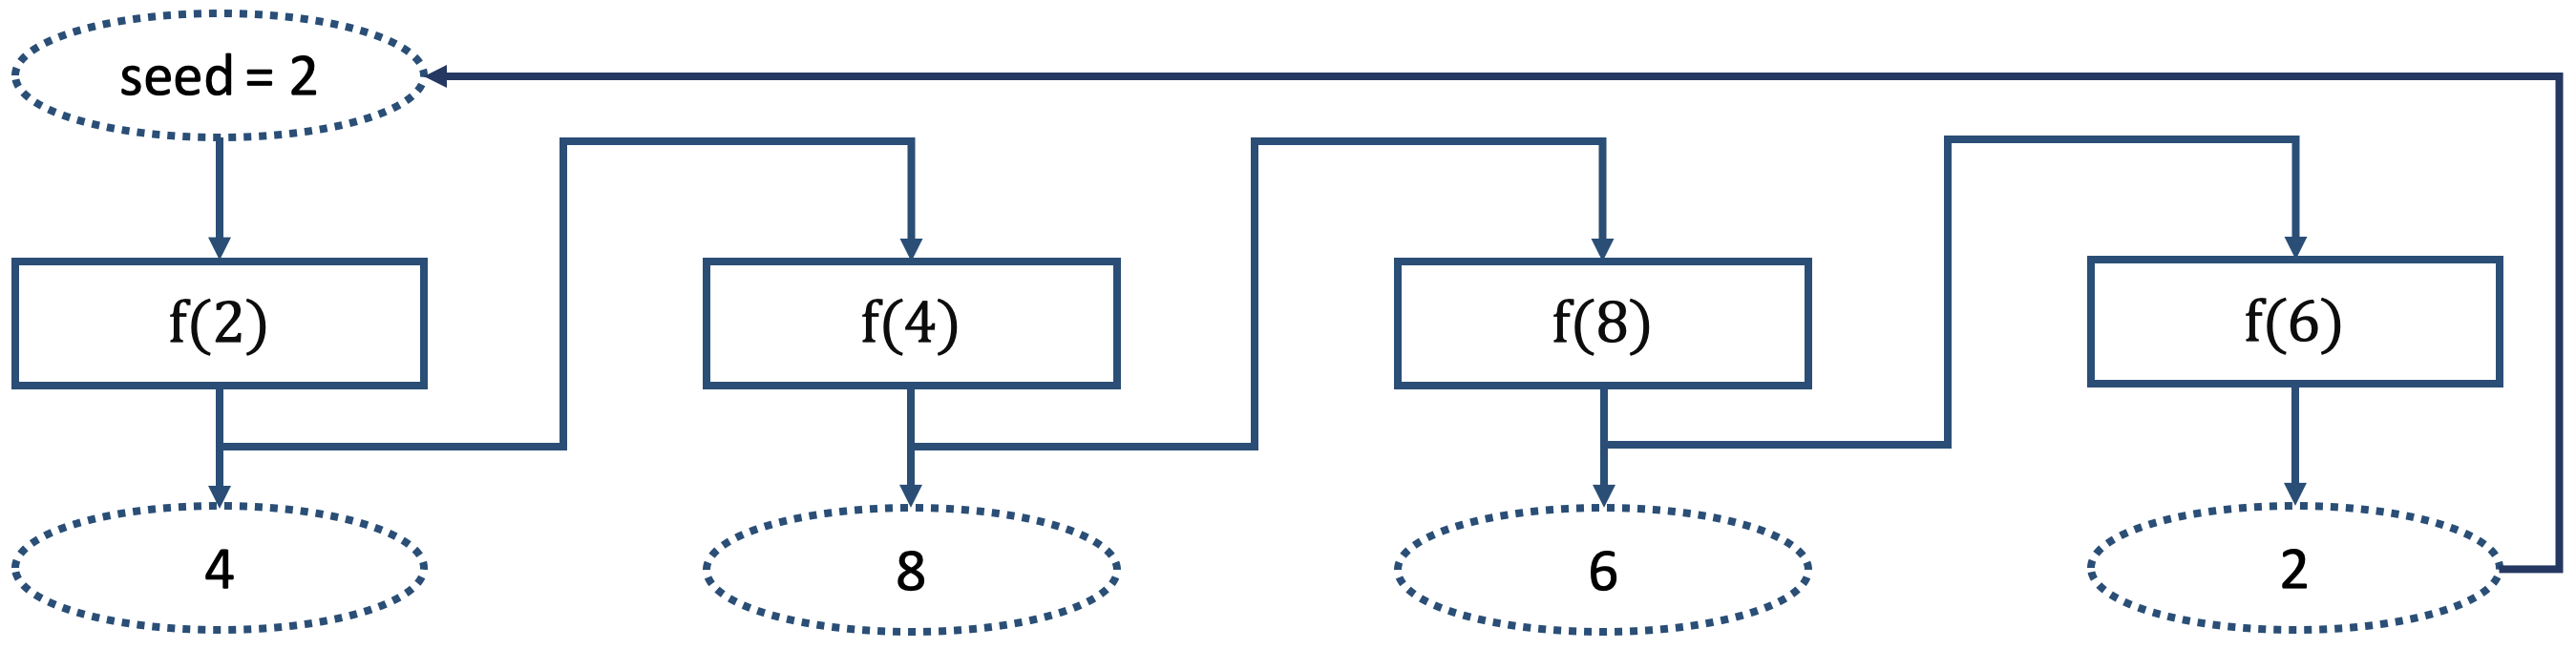
\includegraphics[width=0.8\textwidth]{./images/pictures/prng.png}
	\caption{Example of a schema for the linear congruential pseudo random number generator with the function $f(X) \equiv \left(2 \times X~\bmod~10 \right)$. The period for value of seed 2 is four.}
	\label{fig:prng}
\end{figure}

Since the size of state is fixed, there are finitely many options of inputs and corresponding outputs what eventually leads to repetitions. The number of iterations before the first duplicity is called the \textit{period}. The length of the period is also dependent on a seed. Generators are created so that the \textit{period} is maximized for any seed. When choosing PRNG for an application the \textit{period} should be taken into account; it must be chosen so that the period is never reached. However, this can be achieved by regular reseeding with truly random data. A simple example of a generator run with period four is shown in \cref{fig:prng}.

In fact, modern PRNGs are periodically modifying internal state using truly random data -- those are called hybrid PRNGs. The security is improved by possibility to recover from compromised state, by changing the internal state in a way the attacker cannot predict. However, hybrid PRNGs are deterministic only between two reseedings and consume more truly random data. \cite{krhovjak2009cryptographic}

Since whole sequence generated by PRNG can be determined from the seed, it is important, from security point of view, to keep the seed secret and generate it so that it is unpredictable and truly random.

Sequence produced by PRNG must look random. This means it should also pass all empirical tests of randomness with high probability (covered in \cref{sec:statistical-tests}). \cite{schneier1996applied}

To use PRNG within sensitive applications (such as a cryptographic application), it needs to fulfill one more requirement. It must be unfeasible to compute any information about the previous/following output given that the attacker knows part of the generated sequence, including algorithm and hardware specification. Such generators are called cryptographically secure pseudo-random generators (CSPRNG). \cite{schneier1996applied}

\section{Constructions techniques}

In this thesis, we distinguish between following two categories of PRNGs.

\begin{figure}[h]
	\centering
	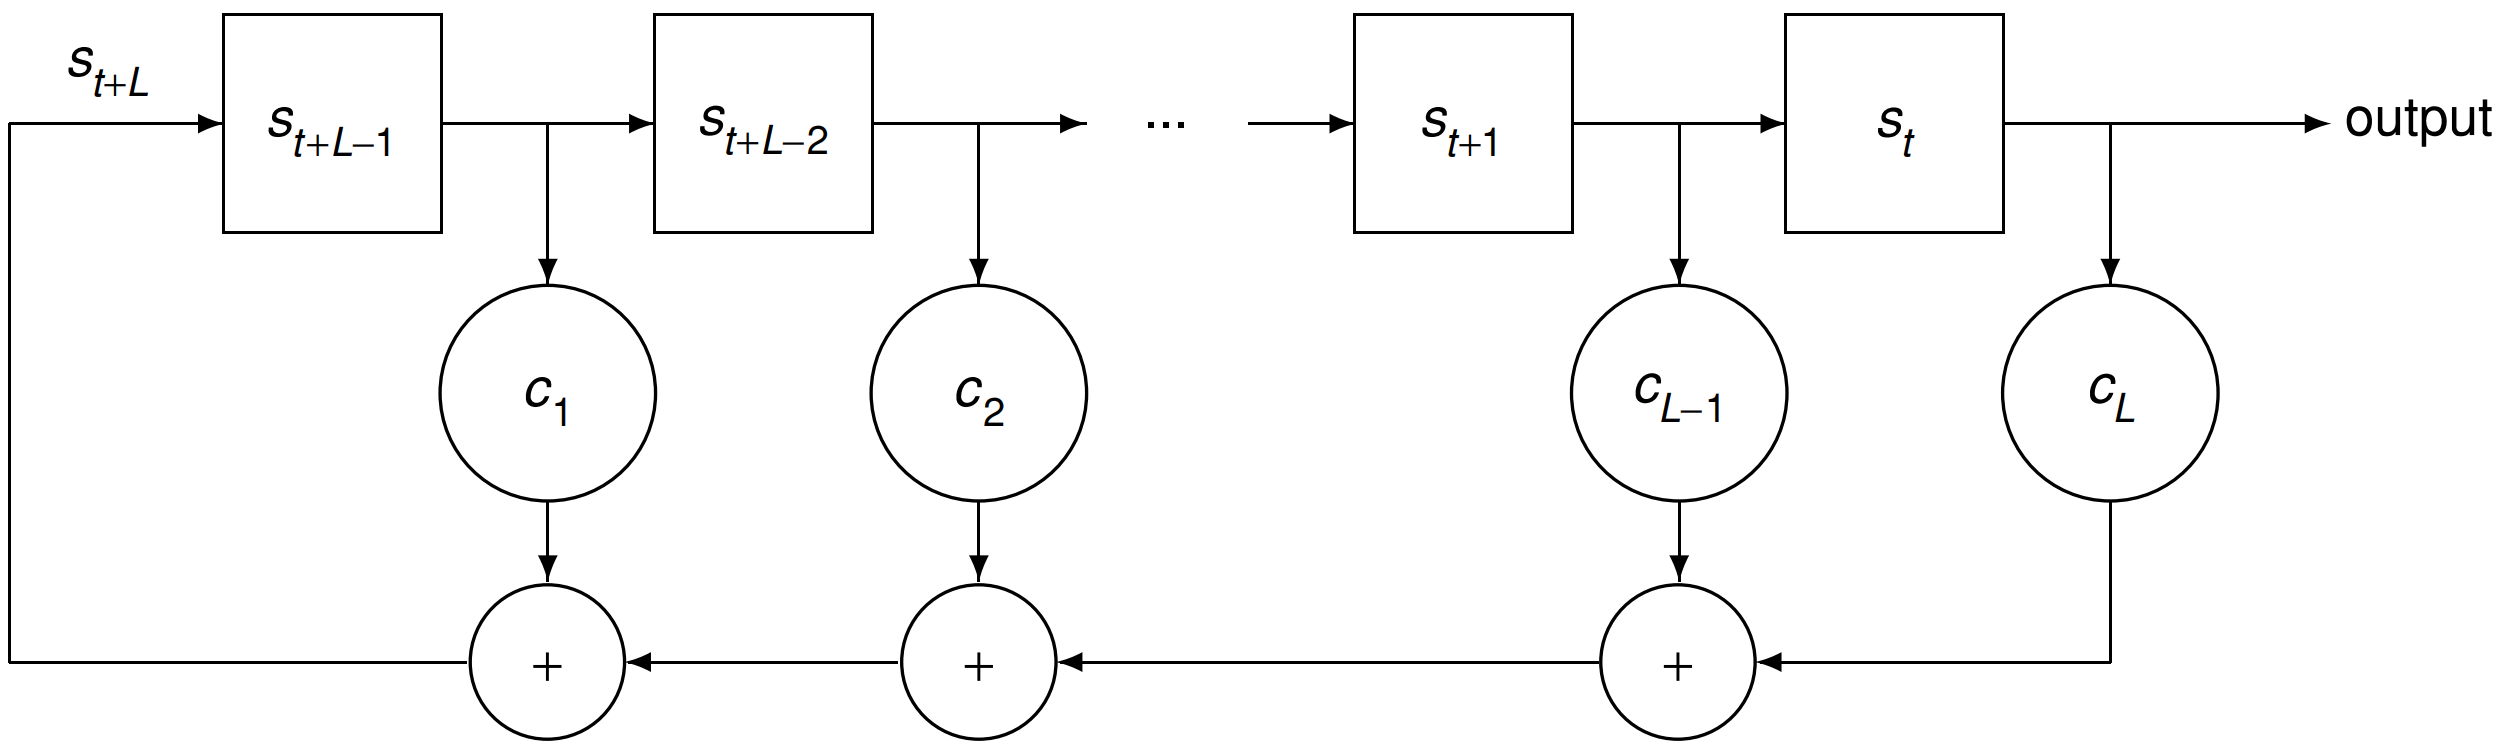
\includegraphics[width=0.8\textwidth]{./images/pictures/lfsr.png}
	\caption{Scheme of Linear Feedback Shift Register. Variable $s$ represents bits of the register and $c$ is parameter of generator. \cite{Canteaut2005}}
	\label{fig:lfsr}
\end{figure}

\begin{description}
	\item[Simple (pure) generators.] The function $f$ is mostly some simple mathematical formula. A commonly known generator of this type is the linear congruential generator (LCG). The formula is following. \cite{LEcuyer07testu01}
	
	\begin{equation}
	x_{n+1} = \left( a \times x_n + c \right)~~\bmod~~m
	\label{formula:lcg}
	\end{equation}	
	

Where \textit{a, c, m} are fixed parameters for specific generator. Simple example of LCG with $a = 2$, $c = 0$ and $m = 10$ is shown in \cref{fig:prng}.

Another basic principle which is a base for lots of generators is a Linear Feedback Shift Register (LFSR). LFSRs are also suitable for hardware implementation, what is one of its advantages. The principle is based on a register which is right shifted every iteration, where rightmost bit is output. The new value for the leftmost bit is determined based on values of other chosen bits within the register. \cref{fig:lfsr}~shows a schema for LFSR. The formula for computation new leftmost bit is following:

\begin{equation}
s_{t + L} = \sum_{i = 1}^{L} c_{i}s_{t + L - i}~~~~~~~~~~~~~~\forall t \geq 0, 
\end{equation}

where $t$ determines a time, $s$ stands for register bit values, and $c$ is a parameter which decides whether $i$-th bit is used for determination of the value of the new bit (leftmost). $L$ represents the bit size of the register. \cite{Canteaut2005}

Makoto Matsumoto and Takuji Nishimura introduced Mersenne Twister pseudo-random generator ~\cite{Matsumoto:1998:MTE:272991.272995} in 1998. It is an extended version of TGFSR~\cite{matsumoto1992twisted} (twisted generalized feedback shift register) algorithm. Despite the long period of length $2^{19937} - 1$, Mersenne twister itself is not cryptographically secure PRNG. However, it is possible to create CSPRNG from MT, for example by modifying output by a hashing algorithm. One of the usages suitable for this generator is within the Monte Carlo simulations. 

\item[PRNGs based on cryptographic primitives.] Even though cryptographic primitives, such as block ciphers or hash functions, are used for different purposes than PRNGs, they have a partly similar objective -- to produce a seemingly random sequence from an input. Therefore, each cryptographic primitive can be easily used for the generation of pseudo-random sequences. The security of resulting generator should be proportional to the security of used primitive. However, to obtain CSPRNG, it is not sufficient that cryptographic primitive produce output with good randomness properties (output is indistinguishable from a truly random stream). PRNG schemes need to guarantee that it is unfeasible to compute previous/next value given part of a generated sequence. In this thesis, we are analyzing output from PRNGs for indistinguishability from truly random sequences. In our analysis, we are testing output directly from cryptographic primitives as they are in most cases providers of pseudo-randomness for this type of generators.

\begin{figure}[h]
	\centering
	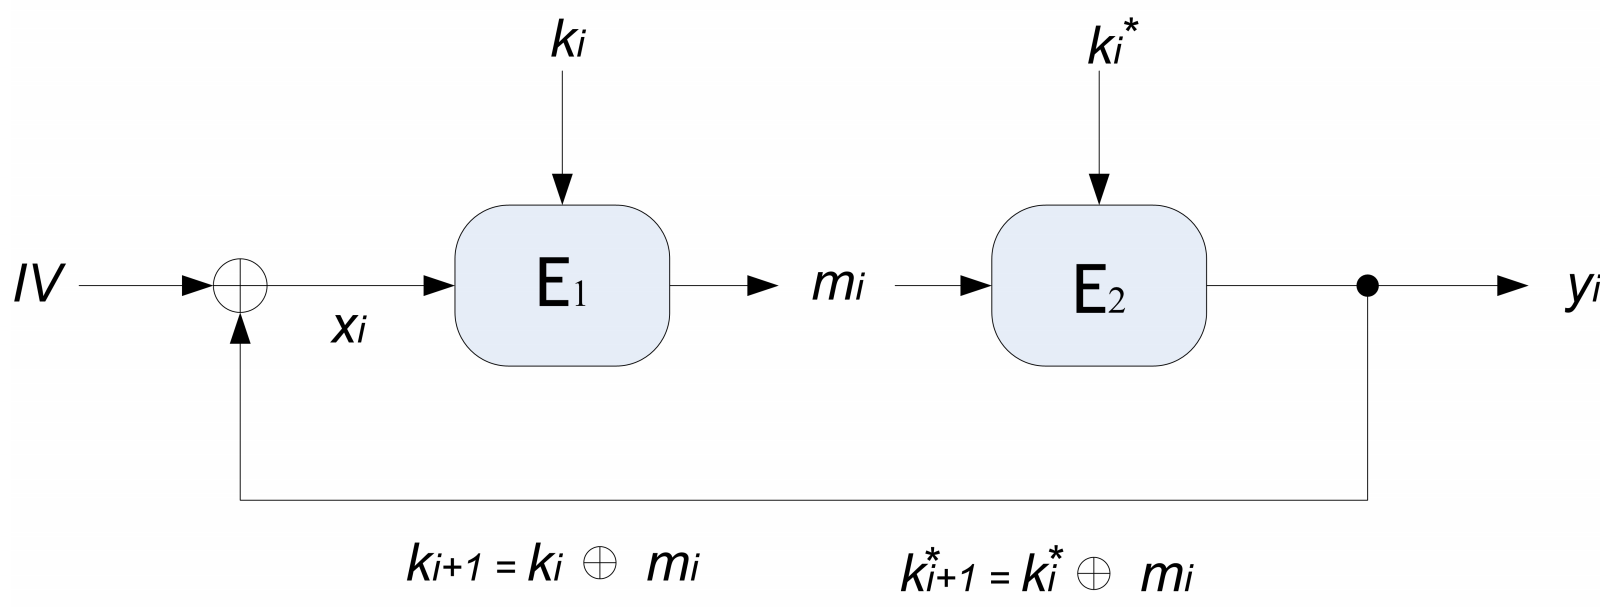
\includegraphics[width=0.5\textwidth]{./images/pictures/block-cipher-prng.png}
	\caption{Example of PRNG created from block cipher taken from \cite{Petit:2008:BCB:1368310.1368322}.}
	\label{fig:block-prng}
\end{figure}

There are multiple additional parameters for creating a PRNG based on a primitive. For block ciphers, one needs to solve what to input to the cipher in each iteration (for example using counter from the value of seed, or chain iterations) and what to use as a key (either use a fixed key or determine the key from an internal state). Christophe Petit et al. studied \cite{Petit:2008:BCB:1368310.1368322} a security of a generator shown in \cref{fig:block-prng}. The studied generator is using two instances of a block cipher. Keys are changed for every iteration and output from $i$-th iteration is used as an input to $(i + 1)$-th iteration.

ANSI X9.17/ANSI X9.31 (\cref{fig:x9-17}) \cite{ansi1985american} introduced standardized way how to turn block cipher into PRNG. This generator could be used with any cryptographic primitive as a provider of pseudo-randomness, however, recommended are 3-DES and AES \cite{Keller05nist-recommendedrandom}.

Regarding hash functions, Russell Impagliazzo et al. proved \cite{Impagliazzo:1989:PGO:73007.73009} that the existence of one-way functions is necessary and sufficient for the existence of pseudo-random generators. 

\end{description} 


\begin{figure}[h]
	\centering
	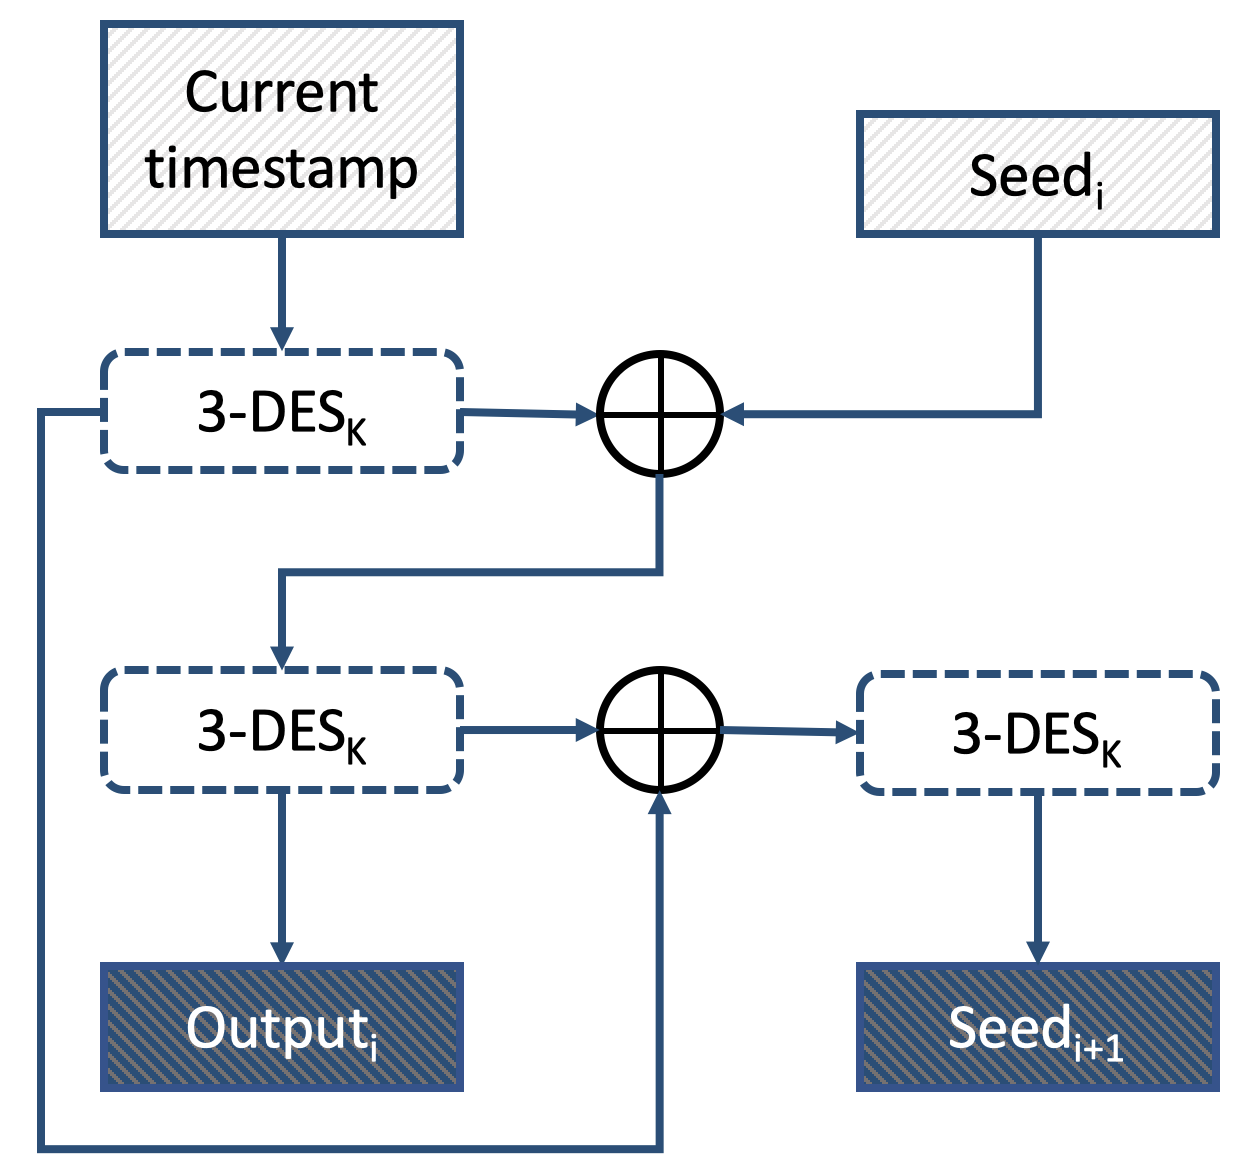
\includegraphics[width=0.5\textwidth]{./images/pictures/x9-17-prng.png}
	\caption{Scheme of ANSI X9.17 PRNG \cite{ansi1985american,kelsey1998cryptanalytic}.}
	\label{fig:x9-17}
\end{figure}

\section{Usage of PRNGs in cryptography}

CSPRNGs in cryptography are used for several purposes, for example, for generation of keys, initialization vectors, but also for encryption and decryption within symmetric cryptography. In this section, closer look to the last usage is presented.

Shannon theorized~\cite{perfect-secrecy} that it is possible to achieve a perfect secrecy only in case a number of possible keys is greater or equal to a number of possible messages. Perfect secrecy means that there is no information about plaintext in ciphertext. The one-time pad cryptosystem achieves this property by having the key longer than message. For encryption, it uses simple bit by bit \texttt{XOR} of plaintext with a large truly random non-repeating sequence as a key. However, distribution of such key is complicated, and in case there would be schema for exchange of such key in secure way, it could be used for sending message itself. \cite{schneier1996applied}

Stream ciphers were introduced with a similar principle in mind as the one-time pad. However, instead of using a long truly random sequence as a key, an output from CSPRNG is used. The ciphertext $C$ is created from plaintext $P$ and keystream (generated from CSPRNG) $K$ as follows: $C_{i} = P_{i} \oplus K_{i}$, for each bit in plaintext. For an encrypted communication both sides need to know the key, which is nothing else than a seed for CSPRNG, to produce the same keystream (for more information see \cite{schneier1996applied}). Stream ciphers are useful for long streams (such as audio or video streams), especially for their zero error propagation. This means if one bit is flipped during a data transfer over the network, only one bit is flipped in decrypted plaintext. For example, if the same situation occurs when using a block cipher in CBC mode whole block is broken after decryption.

\begin{figure}[!h]
	\centering
	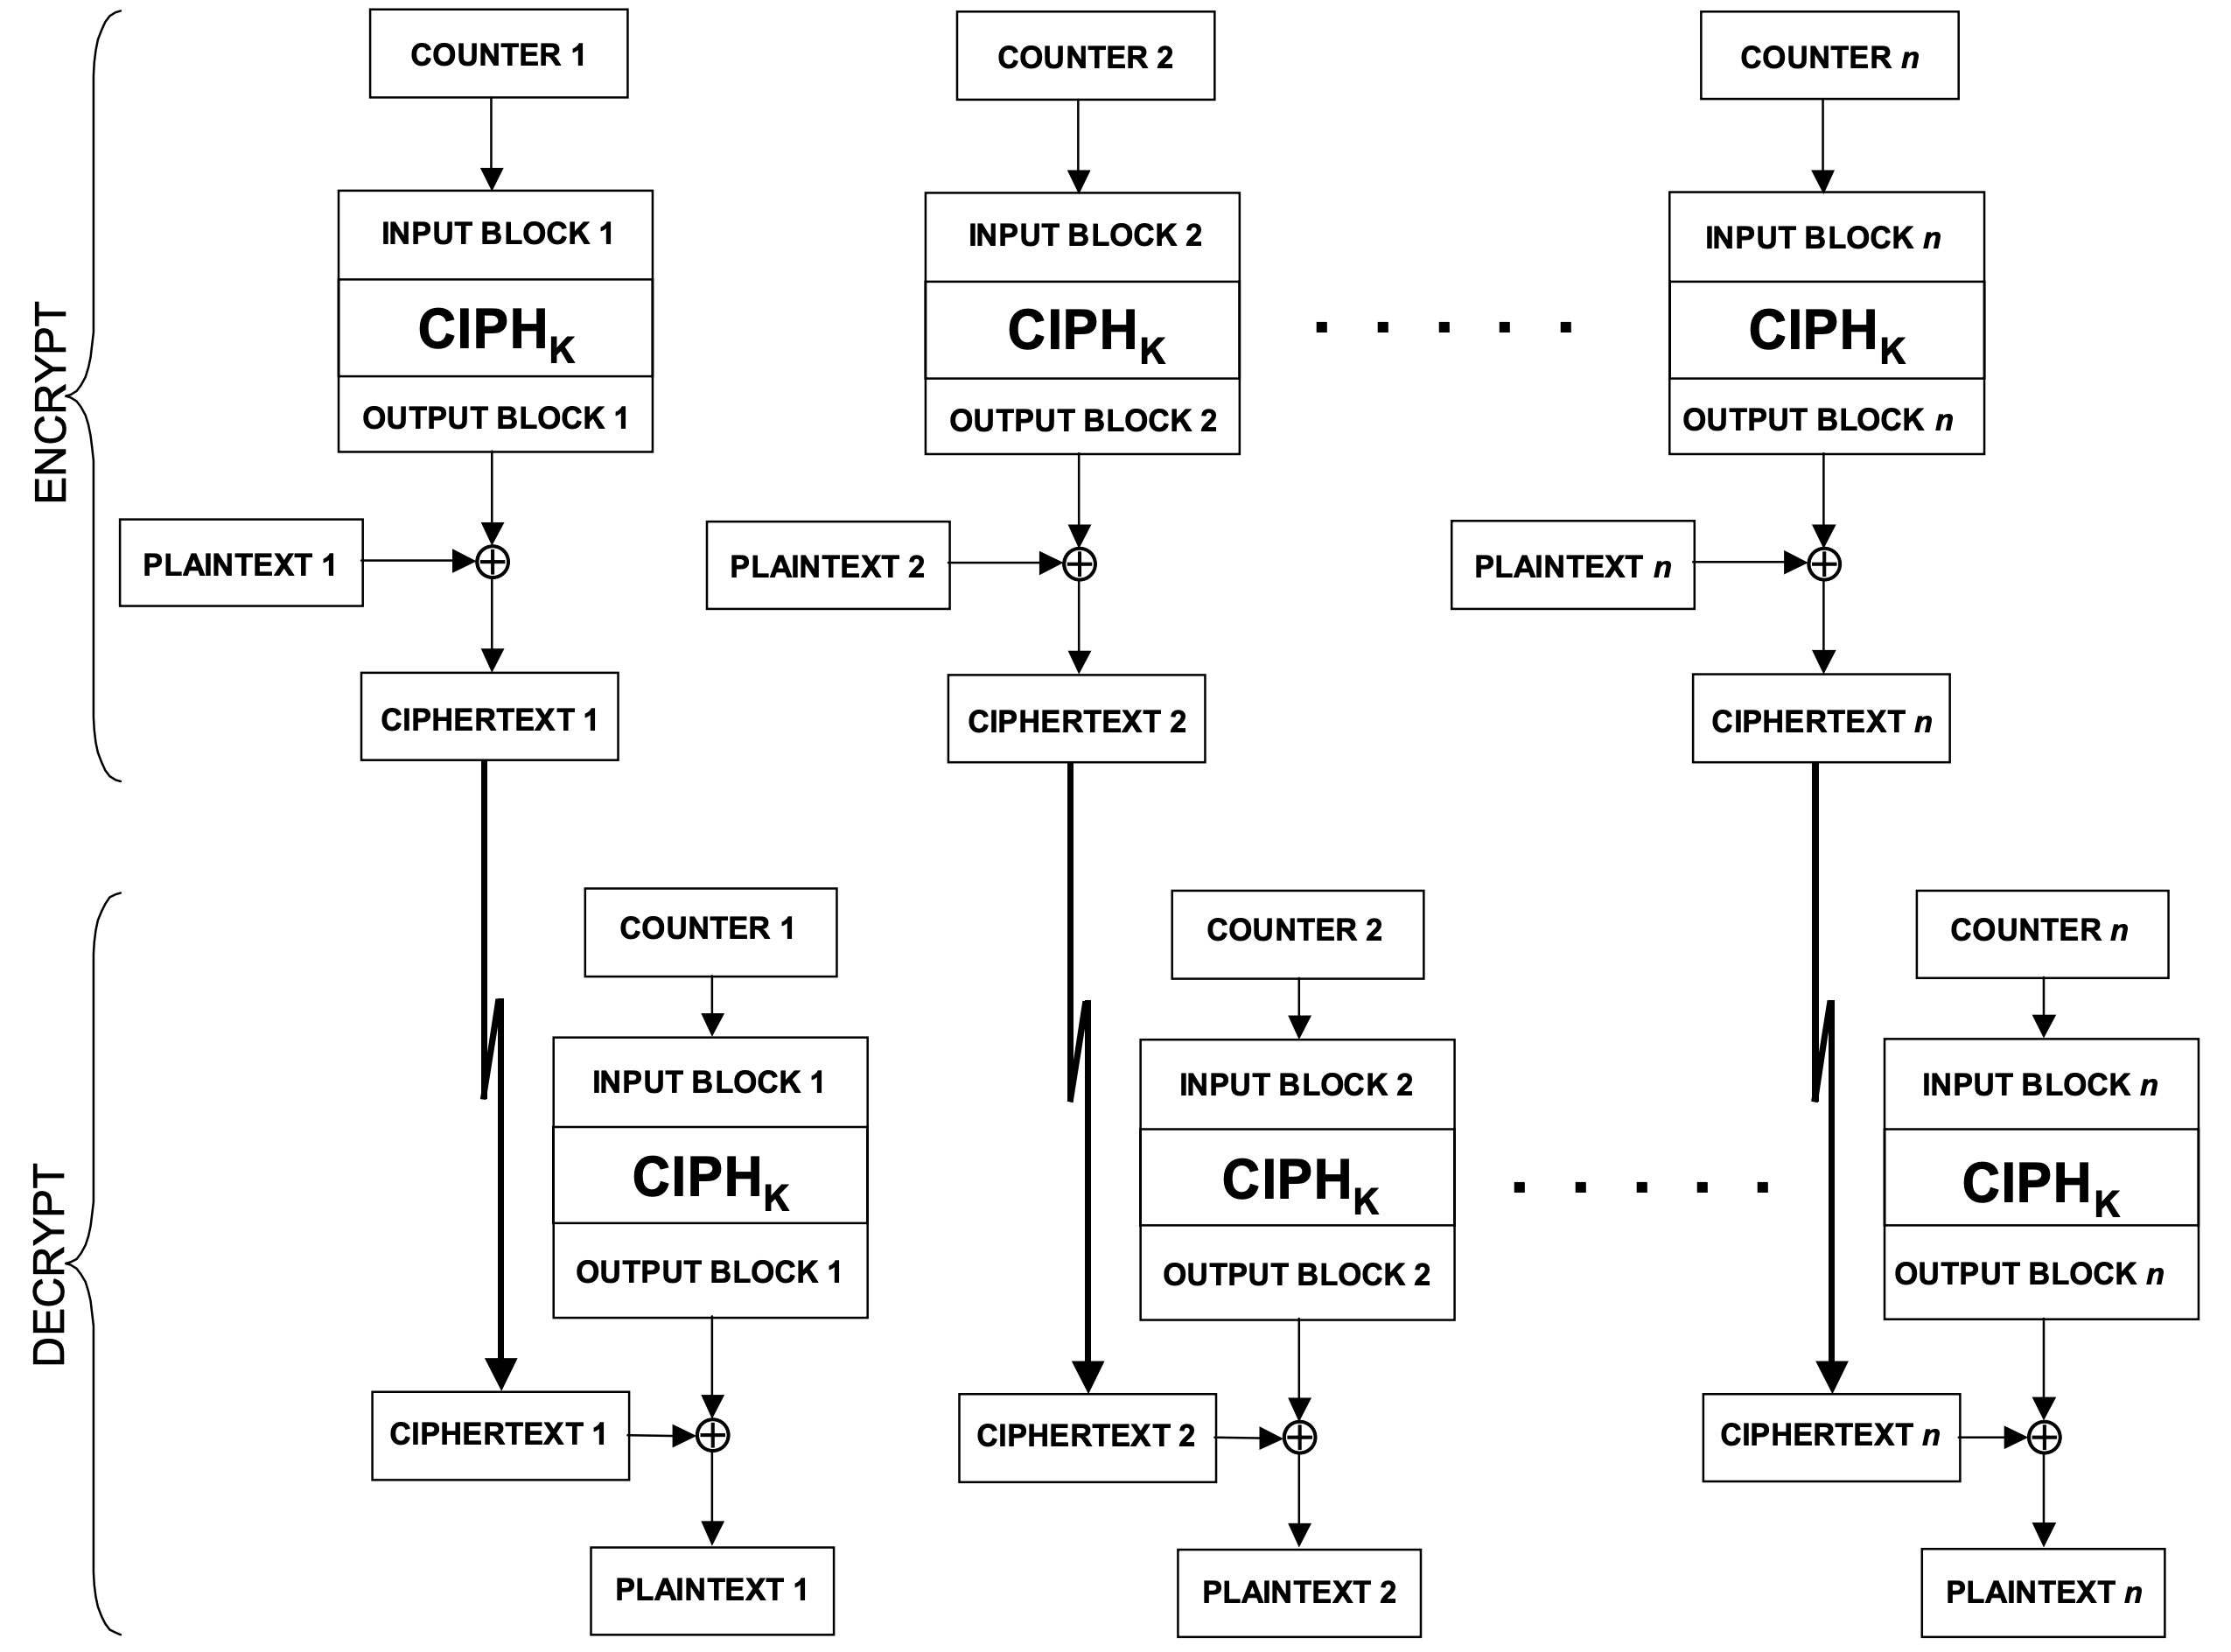
\includegraphics[width=0.6\textwidth]{./images/pictures/ctr.png}
	\caption{Scheme of CTR mode of operation for block ciphers. \cite{Dworkin:2001:SER:2206247}}
	\label{fig:ctr}
\end{figure}

However, block ciphers can act similarly to stream ciphers. For example, in Output Feedback mode (OFB) or Counter mode (CTR) of operation for block ciphers, the plaintext never go through the cipher itself. Cryptographic primitive, in this case, serves only as a generator of a keystream which is \texttt{XOR}-ed with plaintext, similarly like in stream ciphers. \cref{fig:ctr} shows scheme of CTR mode.\cite{Dworkin:2001:SER:2206247}

\section{Typical attacks}

In this section, three theoretical types of attacks against PRNGs are presented which were originally explained by Kelsey et al. in \cite{kelsey1998cryptanalytic}, followed by practical example of attack which were conducted on real generator. Some of those types are similar to attacks conducted within this thesis, see \cref{sec:conducted-experiments}.

\textit{Direct Cryptanalytic Attack} -- analysis of output without any other knowledge of PRNG. For example, distinguishing between truly random data and output from PRNG, more in \cref{sec:statistical-tests}.

\textit{Input-Based Attack} -- an attacker is trying to take advantage of knowing (known-input) or controlling (chosen-input, replayed-input) input to be able to distinguish between outputs from PRNG and truly random generator. Those types of attacks may occur when an insufficient source of entropy is used for generating seed for PRNG such as hard drive latency (possibly observable -- known input), network statistics (may be manipulated by an attacker -- chosen-input/replayed-input). Examples of this type of attacks are conducted in practical part of this thesis, details explained in \cref{sec:conducted-experiments}.

\textit{State Compromise Extension Attack} -- the assumption for this type of attack is that an attacker successfully compromised internal state $S$ of an attacked generator. This might occur for example in a situation where a computer starts from some insecure state. The attack succeeds in case an attacker (with knowledge of $S$) can recover some information about the previous or the next output (either determine output values or distinguish it from truly random data). 

Kesley et al. \cite{kelsey1998cryptanalytic} also analyzed resistance of some real-world PRNGs concerning all mentioned types of attacks. The conclusion for X9.17 PRNG, shown in \cref{fig:x9-17}, is following.

\begin{itemize}
	\item Direct cryptanalysis seems to be equivalent to cryptanalysis of used block cipher (3-DES). However, they didn't prove it.
	
	\item There is a weakness concerning the replayed-input attack. By freezing the time (current time-stamp is the same for every run) it is possible to reduce difficulty to break PRNG from $2^{63}$ to $2^{32}$.
	
	\item Compromising internal state, especially 3-DES encryption key, leads to the destruction of the security; the PRNG itself never recovers from this state. The only way how to recover is generation of whole new state including 3-DES encryption key.
\end{itemize}

Berry Schoenmakers and Andrey Sidorenko conducted practical cryptanalysis \cite{practical-cryptanalysis} against The Dual Elliptic Curve Pseudorandom Generator (DEC PRG)\cite{barker2007recommendation}. The algorithm is based on elliptic curves. The generator in each iteration outputs 240 least significant bits of x coordinate of a point on the elliptic curve. Let $\phi (r)$ denote the number of points on the elliptic curve which have 240 least significant bits equal to $ r $ (size of $ r $ is 240 bits). On used elliptic curve there is close to $2^{256}$ points, this means the expected $\phi (r)$ for any $ r $ which is uniformly distributed is equal to $2^{256 - 240} = 2^{16}$. 

However, Berry Schoenmakers and Andrey Sidorenko found out that for $ r $ generated by DEC PRG the value of $\phi (r)$ is slightly higher than $2^{16}$. Using that knowledge, it is possible to construct distinguisher which can observe this bias between the output from DEC PRG and uniformly distributed data. The distinguisher works as follows: let $ r $ be 240 bits from analyzed data, compute $\phi (r)$, then if the value is higher than $2^{16}$ the output is considered an output from DEC PRG. The probability that output $ r $ from DEC PRG is distinguished by this distinguisher is approximately $ p = 0.50078 $. However, this probability can be improved by computing $\phi$ for k (k > 1) subsequent 240-bit blocks and take the average of those values. The probability of success for attack with $ k = 4000 $ is $ p = 0.548785 $.

\section{Human cryptanalysis}

This section presents two cryptanalysis techniques - a linear and differential cryptanalysis. Both of them are powerful; however, they are not fully automated. The cooperation with cryptanalyst is necessary. The first was introduced by Matsui \cite{matsui1993linear} in 1993 as a theoretical attack on Data Encryption Standard (DES). The other was proposed by Biham and Shamir \cite{Biham1991} in 1991 with the same objective, to attack DES.


\subsection{Linear cryptanalysis}

It is one of the most famous known plaintext attacks against block ciphers; the assumption is that an attacker knows some number of plaintext/ciphertext pairs, but he is not able to choose specific ones. 

The attack is based on building a linear approximation of part of a block cipher (non-linear), which consists of bits of plaintext, ciphertext, and key (round subkey). The general form of such approximation is following: 
\begin{equation}
\left( \bigoplus_{i \in \{1...b\}} P_{i} \right) \oplus \left( \bigoplus_{j \in \{1...b\}} C_{j} \right) = \left( \bigoplus_{k \in \{1...s\}} K_{k} \right)
\label{eq:general_approx}
\end{equation}
where $P_{i}$, $C_{j}$ and $K_{k}$ denote $i,j,k$-th bit of plaintext, ciphertext and key respectively. $\oplus$ stands for Boolean \texttt{XOR} operator. Variables $b$ and $s$ are function-specific and represent block size and key size. \cite{junod2000linear} 

Given such approximation and a perfect cipher, the probability that this approximation holds should be on average $p = \frac{1}{2}$. Probability $p$ can be computed from the structure of the investigated function. For purposes of the attack we need to find an approximation which maximizes the bias $\epsilon = \lvert p - \frac{1}{2} \rvert$. 

The linear approximation can be used to perform two types of attacks:

\begin{description}
	\item[Obtaining one-bit information about the key.] Given the approximation in the form of \cref{eq:general_approx}, it is possible to obtain one-bit value of $X = \left( \bigoplus_{k \in \{1...s\}} K_{k} \right)$ following \cref{alg:one-bit}. \cite{junod2000linear}
	
	\begin{algorithm}[H]
		\KwData{$T$ denotes the number of results which equal to 0 when computing value of approximation for $N$ plaintext/ciphertext pairs.}

		\eIf{$T > \frac{N}{2}$}{

			$X = \begin{cases}
					0, & p > \frac{1}{2} \\
					1, & \text{otherwise}
				\end{cases}
			$
		}{
			$X = \begin{cases}
					1, & p > \frac{1}{2} \\
					0, & \text{otherwise}
				\end{cases}
			$
		}
		
		\caption{Obtaining one bit information about the key using the linear approximation.} 
		\label{alg:one-bit}
	\end{algorithm}
	
	\item[Obtaining more bits of the key.] For demonstrating this type of attack, we follow the tutorial from \cite{human-cryptanalysis} published by Howard M. Heys. He is attacking Substitution Permutation Network (SPN) defined within this paper. This function has four rounds; the size of subkey for each round and block is 16 bits. Each round consists of these operations: \texttt{mixing with subkey}, \texttt{substitution}, \texttt{permutation}. There are five subkeys because last round contains one more \texttt{mixing with subkey} at the end. Used notation is following.
	
	\begin{itemize}
		\item $K_{k,i}$ is an $i$-th bit of subkey for a $k$-th round. ($k \in \{1..5\}, i \in \{1..16\}$)
		\item $V_{j,i}$ is an $i$-th bit of output of a $j$-th round. ($j \in \{1..4\}, i \in \{1..16\}$)
		\item $U_{l,i}$ is an $i$-th bit of input to an $i$-th round. ($i \in \{1..4\}, i \in \{1..16\}$)
		
		$U_{i} = \begin{cases}
		P \bigoplus K_{1}, & i = 1 \\
		V_{i-1} \bigoplus K_{i}, & \text{otherwise}
		\end{cases}
		$
	\end{itemize}

	Heys is performing attack using 3-round approximation with probability either $p = \frac{15}{32}$ or $p = \frac{17}{32}$ based on specific subkeys. Key bits are omitted from the equation because the \texttt{XOR} of all key bits results into fixed 0 or 1 bit which does not change resulting bias $\epsilon = \frac{1}{32}$. The approximation is following.                 
	
	\begin{equation}
	U_{4,6} \oplus U_{4,8} \oplus U_{4,14} \oplus U_{4,16} \oplus P_{5} \oplus P_{7} \oplus P_{8} = 0
	\label{eq:linear-approximation-heys}
	\end{equation}
	
	Using this formula, it is possible to attack the last subkey $K_5$ by performing steps below.
	
	\begin{enumerate}
		\item Generate all possible options for subkey $K_{5}$ ($2^{16}$).
		\item For each of $N$ collected plaintext/ciphertext pair obtain bits of $U_{4}$ by reversing last round. 
		\item Apply the linear approximation (\cref{eq:linear-approximation-heys}) to captured bits and plaintext.
		\item For each subkey remember the number of pairs the approximation resulted with 0.  
		\item A subkey which ended up with a number which is most significantly different from $\frac{N}{2}$ is considered correct guess.
	\end{enumerate}
\end{description}

Using the linear cryptanalysis Matsui \cite{matsuiAttack} was able to break DES in the full number of rounds using $2^{43}$ random plaintext/ciphertext pairs.

\subsection{Differential cryptanalysis}

It is chosen plaintext attack; an attacker owns some number of plaintext/ciphertext pairs for a fixed unknown key, and he can choose specific plaintexts. 

The attack is based on dependence between differences of two plaintexts and corresponding outputs. Differences are computed using exclusive xor operation of whole block, for example difference between two plaintexts $X_{1}$ and $X_{2}$ is denoted by $\Delta X = X_{1} \bigoplus X_{2}$. The difference between outputs $Y_{1}$ and $Y_{2}$ is expressed by $\Delta Y = Y_{1} \bigoplus Y_{2}$. In ideal case the probability $p$, of getting difference $\Delta Y$ for some  $\Delta X$, should be $\frac{1}{2^{n}}$ (differences should be equally distributed). 

The idea behind the attack is looking for the pair ($\Delta X$, $\Delta Y$) which maximizes the probability $p$ of obtaining difference $\Delta Y$ for plaintext $\Delta X$. The pair ($\Delta X$, $\Delta Y$) is called \textit{differential}.

Heys in his tutorial \cite{human-cryptanalysis} was simulating an attack using differential analysis with three round \textit{differential} ($\Delta U_{4}$ stands for a difference between inputs to fourth round). He found out that SPN for the plaintext difference $\Delta P = [0000$ $1011$ $0000$ $0000]$ results with $\Delta U_{4} = [0000$ $0110$ $0000$ $0110]$ with probability $\frac{27}{1024}$. Given this approximation it is possible to obtain bits of $K_{5}$ following steps below.

\begin{enumerate}
	\item Collect N plaintext pairs which satisfy chosen difference $\Delta P$.
	\item Generate all possible options for $K_{5}$ ($2^{16}$).
	\item For each plaintext pair and each option of key do following steps.
	\begin{enumerate}
		\item Reversely compute bits of $U_{4}$ for both corresponding ciphertexts using guessed key.
		\item For each key remember the number of times computed values give expected difference $\Delta U_{4}$.
	\end{enumerate}
	\item A key with the largest computed number is considered correct guess.
\end{enumerate}

DES in full round has been broken with complexity less than $2^{55}$. \cite{Biham1991}

\section{Distinguishers from truly random streams}
\label{sec:statistical-tests}

One of the most important properties of output from cryptographic primitive is its indistinguishability from truly random data. Automatic tools for analyzing cryptographic primitives are based on this fact. Those tools rely on so-called empirical tests of randomness. Each tool contains several tests, where each of them has a different approach to testing. Mostly they are based on some property where there is a high probability that a truly random generator will satisfy this property. By comparing the expected and actual form of data, we can find out \textit{bias}. Higher the bias is, there is less probability that truly random generator outputted tested sequence.

Tests are based on testing a \textit{null hypothesis}, which is mostly formulated as data being tested are random. Those tests are based on probability; this means that even truly random data may end up with rejected hypothesis. The output of each test is called \textit{p-value} which can be described as a probability that a truly random generator produces data which are less random than the data which were tested. We interpret the tests with respect to a significance level which is commonly denoted as $\alpha$. If the resulting \textit{p-value} is less than the significance level we say we rejected the hypothesis on significance level $\alpha$ (data are probably not coming from a truly random generator). The common value of $\alpha$ is 0.01. \cite{nist-explanation}

There are two types of errors which may occur during interpretation, Type I and Type II. Type I means that truly random data were rejected. The probability of Type I error is equal to significance level $\alpha$. When a tool does not reject data from a faulty generator, Type II error occurred. The probability of this error is denoted by $\beta$. However it is complicated to compute the value of $\beta$ because there are many possible types of non-randomness which might occur. \cite{nist-explanation}

The example of the common test often included in statistical test suites is a Monobit test, which is examining the uniformity of distribution of binary zeroes and ones bits within tested data. It is based on the fact, that there is a high probability that the amount of binary ones and zeroes is approximately the same assuming that each sequence occurs with same probability. A high-level view of this test is shown in \cref{fig:monobit}. 

\begin{figure}[h]
	\centering
	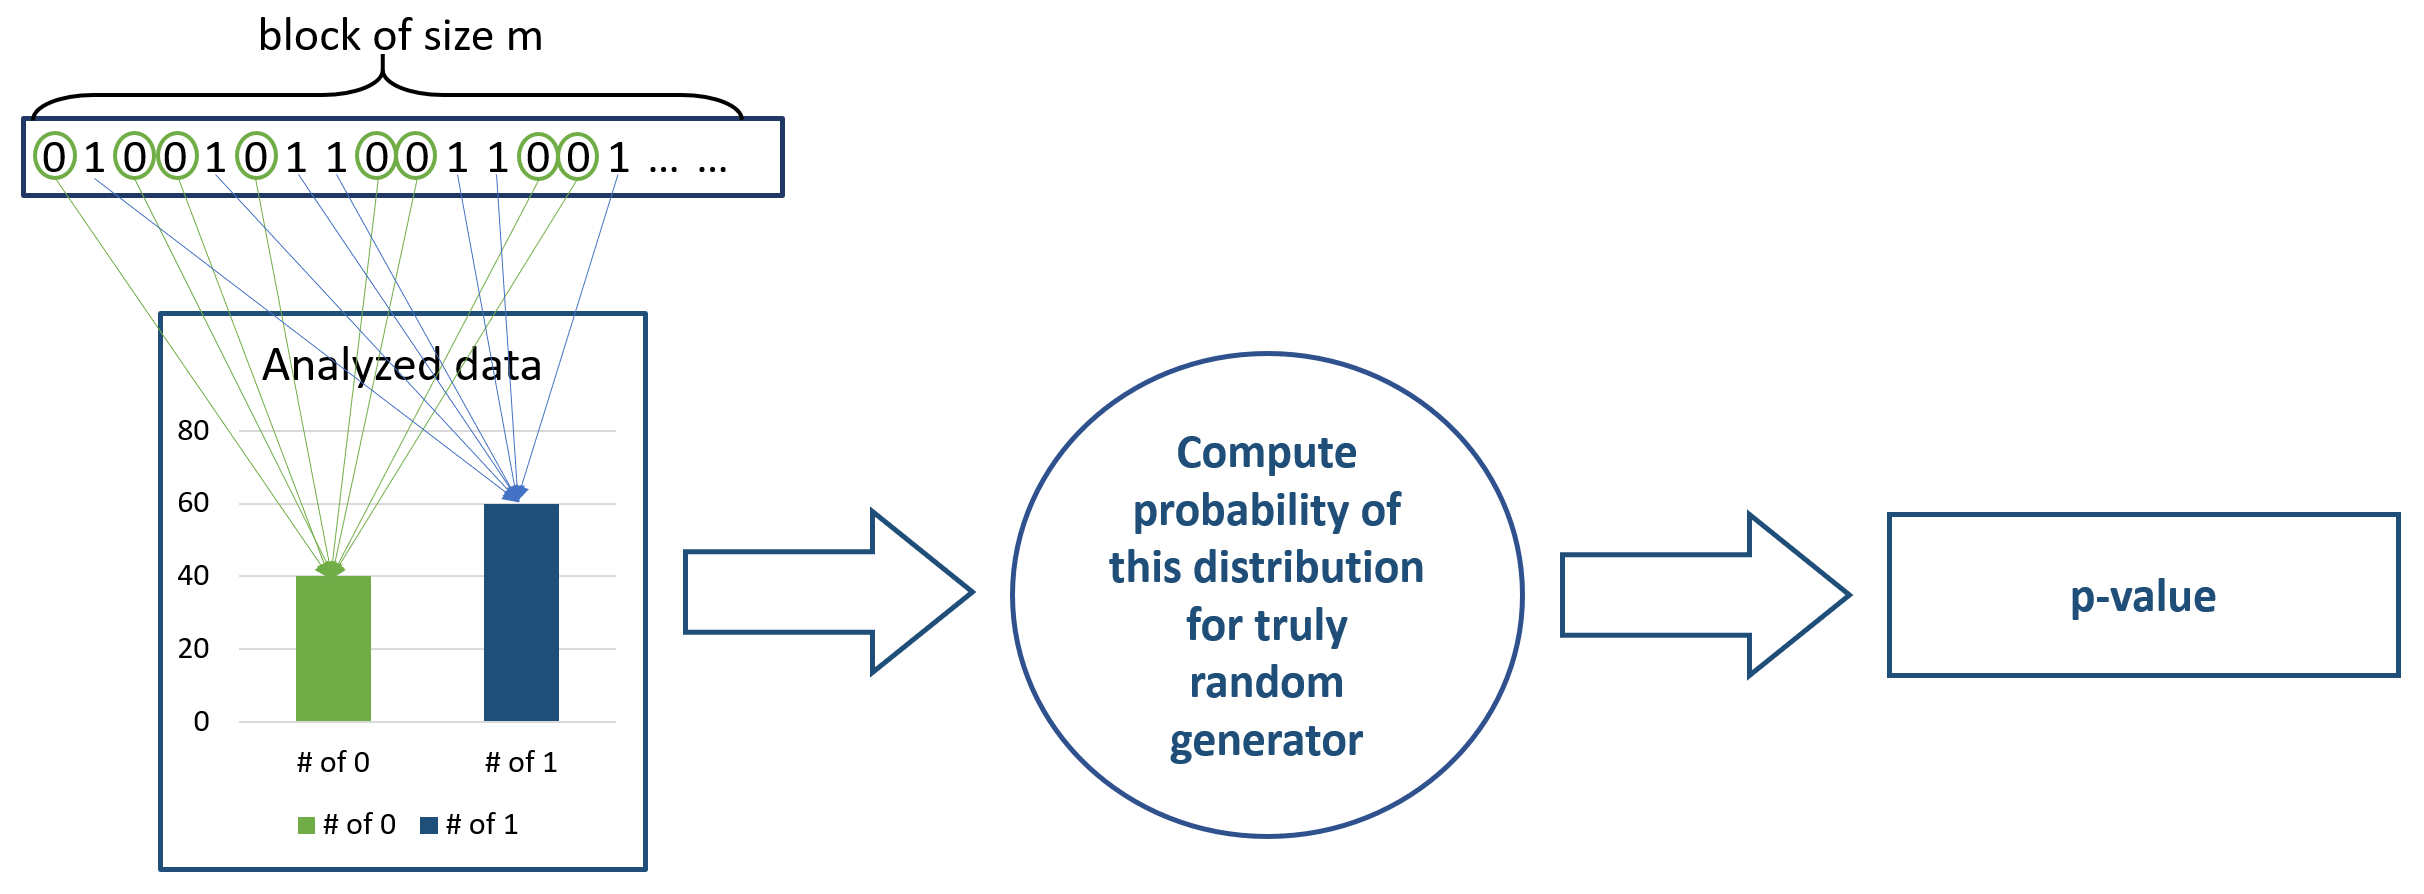
\includegraphics[width=0.9\textwidth]{./images/pictures/monobit-high-level.png}
	\caption{Monobit test from high level point of view.}
	\label{fig:monobit}
\end{figure}

\cref{fig:whole-suite} shows a high-level view of the whole test suite, where all tests are triggered. After evaluation of all tests, it is necessary to interpret the entire run of the battery of tests and make a final decision, whether investigated data are considered truly random or not. It is likely that even data with perfect properties will fail some of the tests due to Type I error. Ľubomír Obrátil conducted \cite{Obratil2017thesis} an extensive analysis on the expectation of a number of failed tests based on a non-trivial number of results for truly random data. Out interpretation is mostly based on his work; however, in some border cases, we were also taking into account an extremeness of p-value of failed tests. Resulting p-value denotes a probability that truly random generator produces a result more extreme than the one which was analyzed. Statistical tools mostly consider a test failed when resulting p-value is less than $ 10^{-4}  $ \cite{nist-explanation,dieharder}. Therefore, when we obtained more tests, but less than expected from analysis of Ľubomír Obrátil, with a p-value less than $10^{-7}$ for output from border round of a function, we considered this sequence as non-random because the probability of this situation is almost impossible.

\begin{figure}[h]
	\centering
	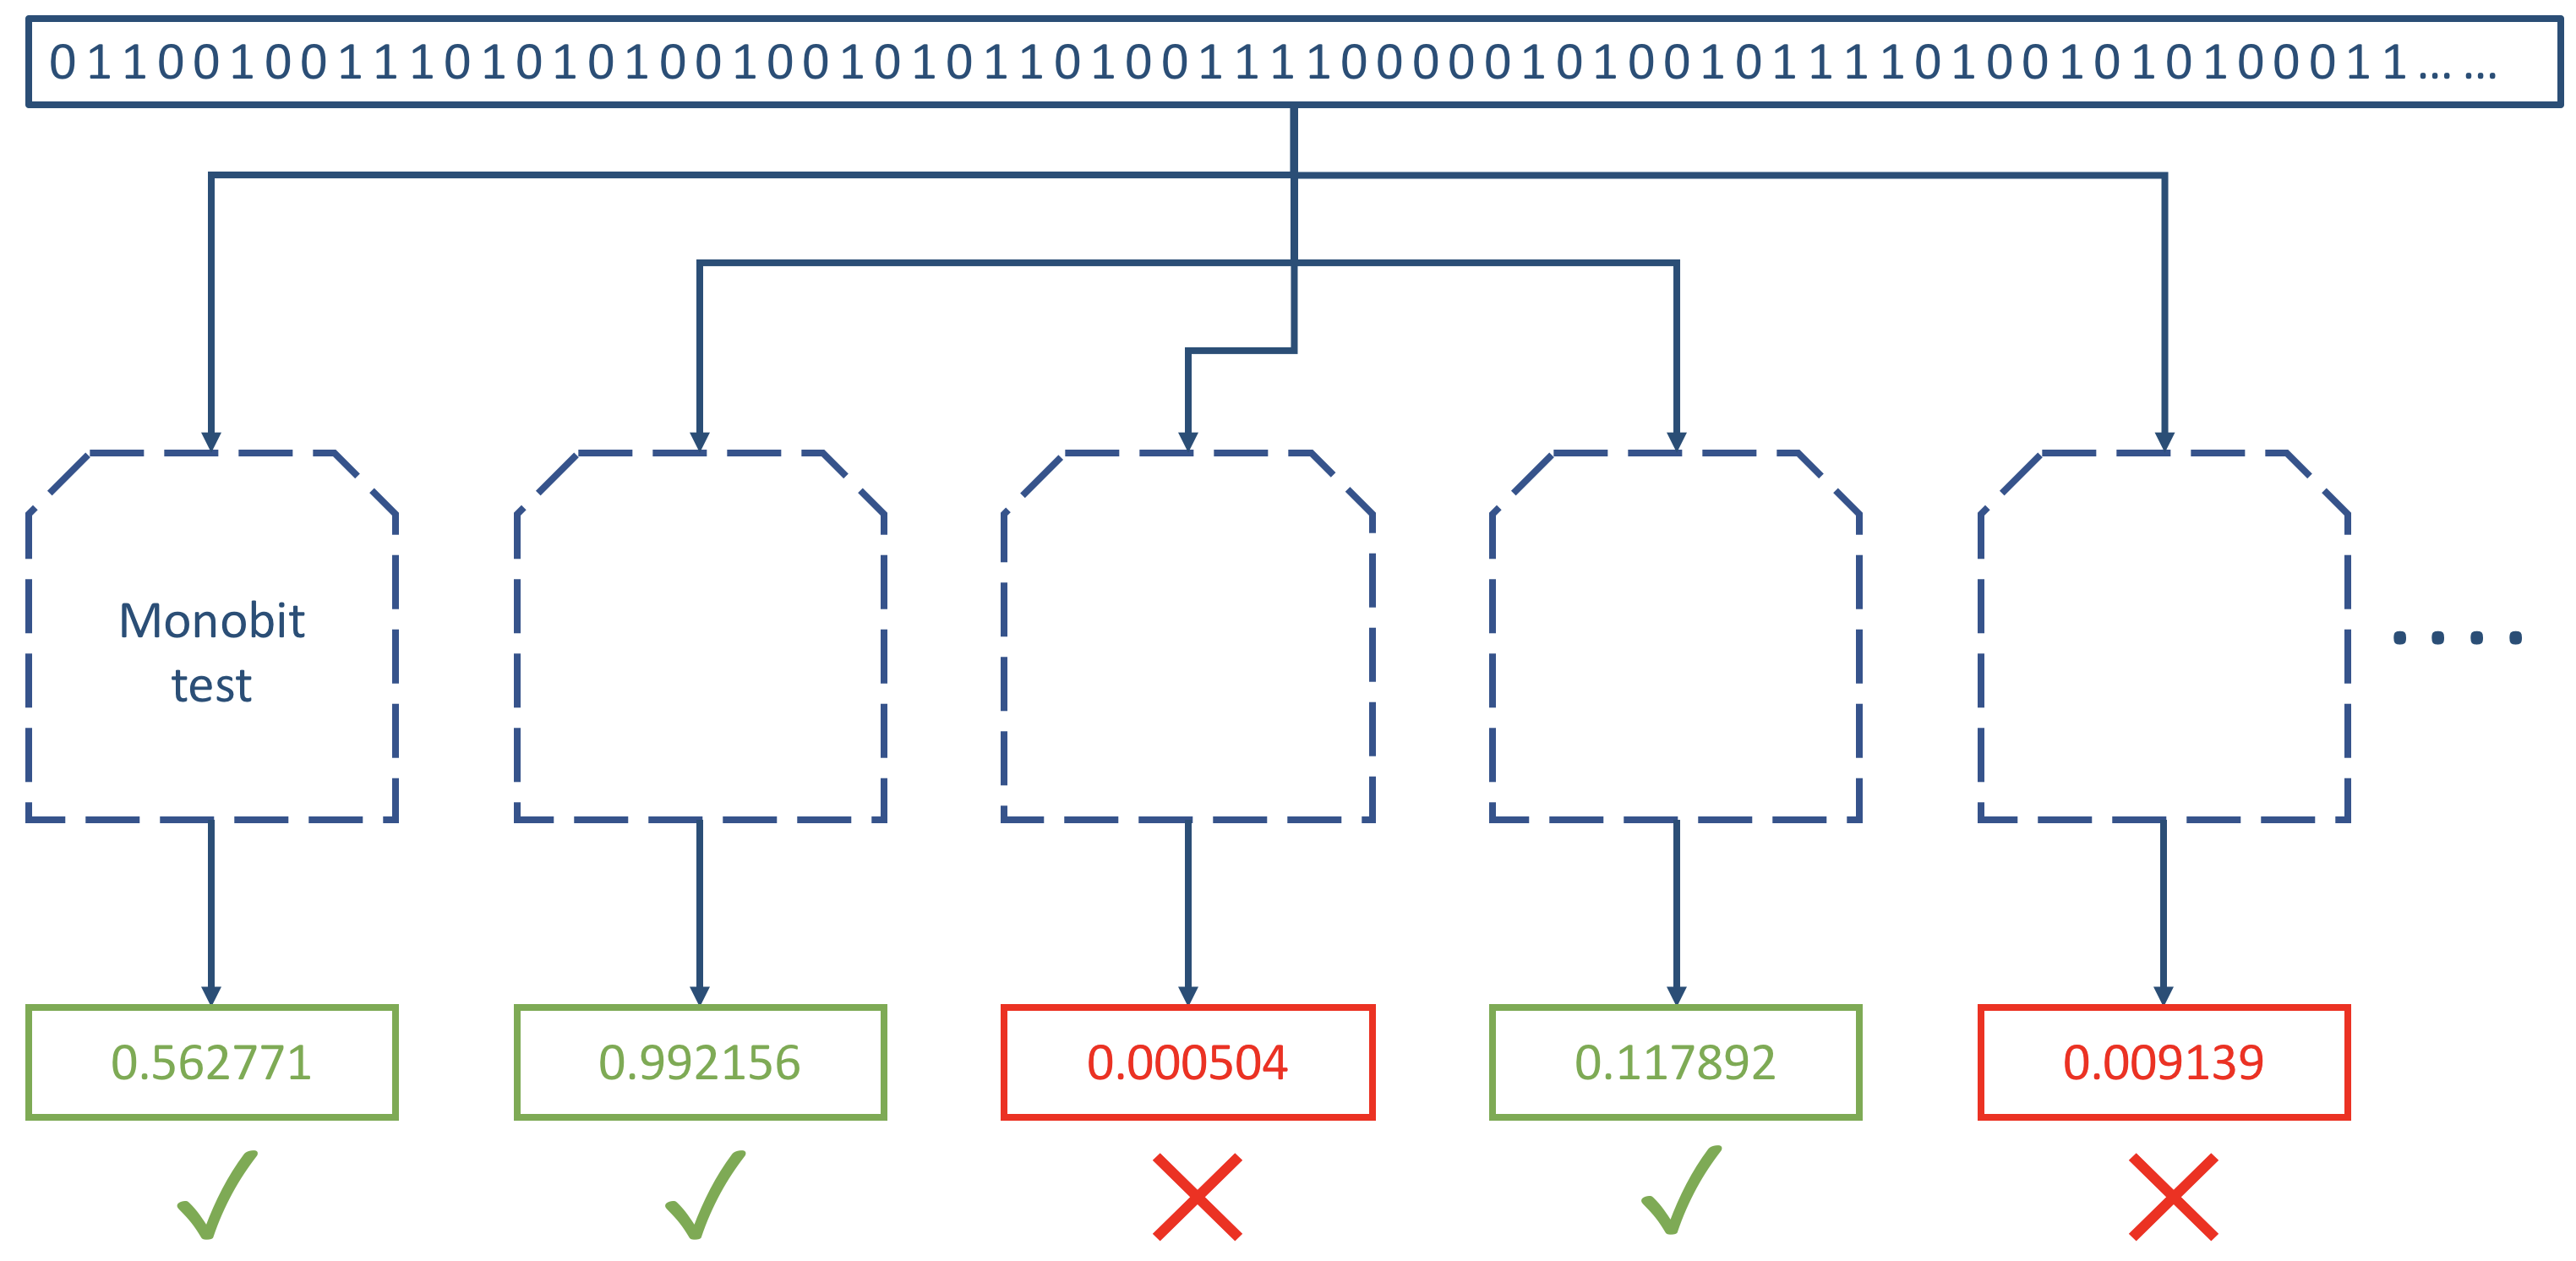
\includegraphics[width=0.9\textwidth]{./images/pictures/software-tool.png}
	\caption{High level view of software tool run.}
	\label{fig:whole-suite}
\end{figure}

\subsection{NIST STS}
{NIST STS}~\cite{nist-sts} is the most commonly used software tool for statistical analysis. It was developed by National Institute Of Standards and Technology (NIST) and is also part of FIPS 140-2~\cite{NIST140-2} certification process. Even though the STS test suite is most commonly used, some of the other test suites generally have better results.

In this thesis we will not use original NIST STS implementation, instead of that we are using optimized version developed Marek Sýs and Zdeněk Říha which is approximately 50 times faster than reference implementation \cite{Sys:2016:A9O:2988516.2988228}. 

The tool contains 15 tests. However several of them have more variants. In total, 188 tests are executed within one run.

\subsection{Dieharder}

Dieharder~\cite{dieharder} is an extension of Diehard test suite \cite{diehard} developed by Robert G. Brown at Duke University. In the newest version, it contains together 31 tests. All tests from Diehard, three originates from NIST STS and the others are implemented by the author or come from different sources. However, not all tests will be used within this thesis. For choosing what tests to run we rely on project Randomness Testing Toolkit~\cite{Obratil2017thesis}.

\subsection{TestU01}

Pierre L'Ecuyer and Richard Simard introduced TestU01 software tool. The aim of this tool is the provision of the general and extensive set of software tools for statistical testing of random number generators. It contains a significant number of tests, more than any other software tool we mentioned. Tests are organized into six batteries of tests. The battery of tests is a subset of tests, where each battery has a different purpose or time consumption. Batteries within TestU01 are divided into two categories, three of them designed for sequences of real numbers and the other for bit sequences.

For the first category there are batteries named \textit{SmallCrush}, \textit{Crush} and \textit{BigCrush}. \textit{SmallCrush} is fastest battery, hence it is recommended to start testing with this one and continue to \textit{Crush} only if sequence pass all tests. \textit{BigCrush} is longest one, it consumes 1414 times more time than \textit{SmallCrush} and 5 times more time than \textit{Crush} to test \textit{Mersenne Twister}~\cite{Matsumoto:1998:MTE:272991.272995} PRNG on a computer with AMD Athlon running at 2.4GHz. For binary sequences there are batteries \textit{Rabbit}, \textit{Alphabit} and \textit{BlockAlphabit}. \cite{l2007testu01}

Besides the batteries this software tool contains also some predefined pseudo-random number generators. Paper~\cite{l2007testu01} contains also results of those generators with batteries \textit{SmallCrush}, \textit{Crush} and \textit{BigCrush}.

\subsection{BoolTest}
\label{sec:booltest-theory}

BoolTest is a simple but strong testing tool developed by Marek Sýs et al. at the Centre for Research on Cryptography and Security, Masaryk University in Brno. It has a slightly different approach to randomness testing. The tool is based on a generalization of Monobit test. The main idea is looking for distinguisher between truly random and tested data in the form of Boolean function. If a distinguisher is found the data are considered non-random. The process starts with a division of sequence into blocks with size \textit{m}. The Boolean function is in the form $f(x_{1}, x_{2}, \cdot \cdot \cdot, x_{m})$. Notice that Monobit test is specific case of this generalization with $m = 1$ and Boolean function $f(x_{1}) = x_{1}$. 

Computation of success of distinguisher requires calculation of the value of the Boolean function for each block so that $x_{k}$ is $k$-th bit of the block.
Expected number of computations which results with binary one is statistically computed and compared with actual results using Z-score statistics \cite{sheskin2003handbook}. From Z-score statistic it is possible to obtain p-value. \cref{fig:bool-test} shows example of evaluation of success of distinguisher.

\begin{figure}[h]
	\centering
	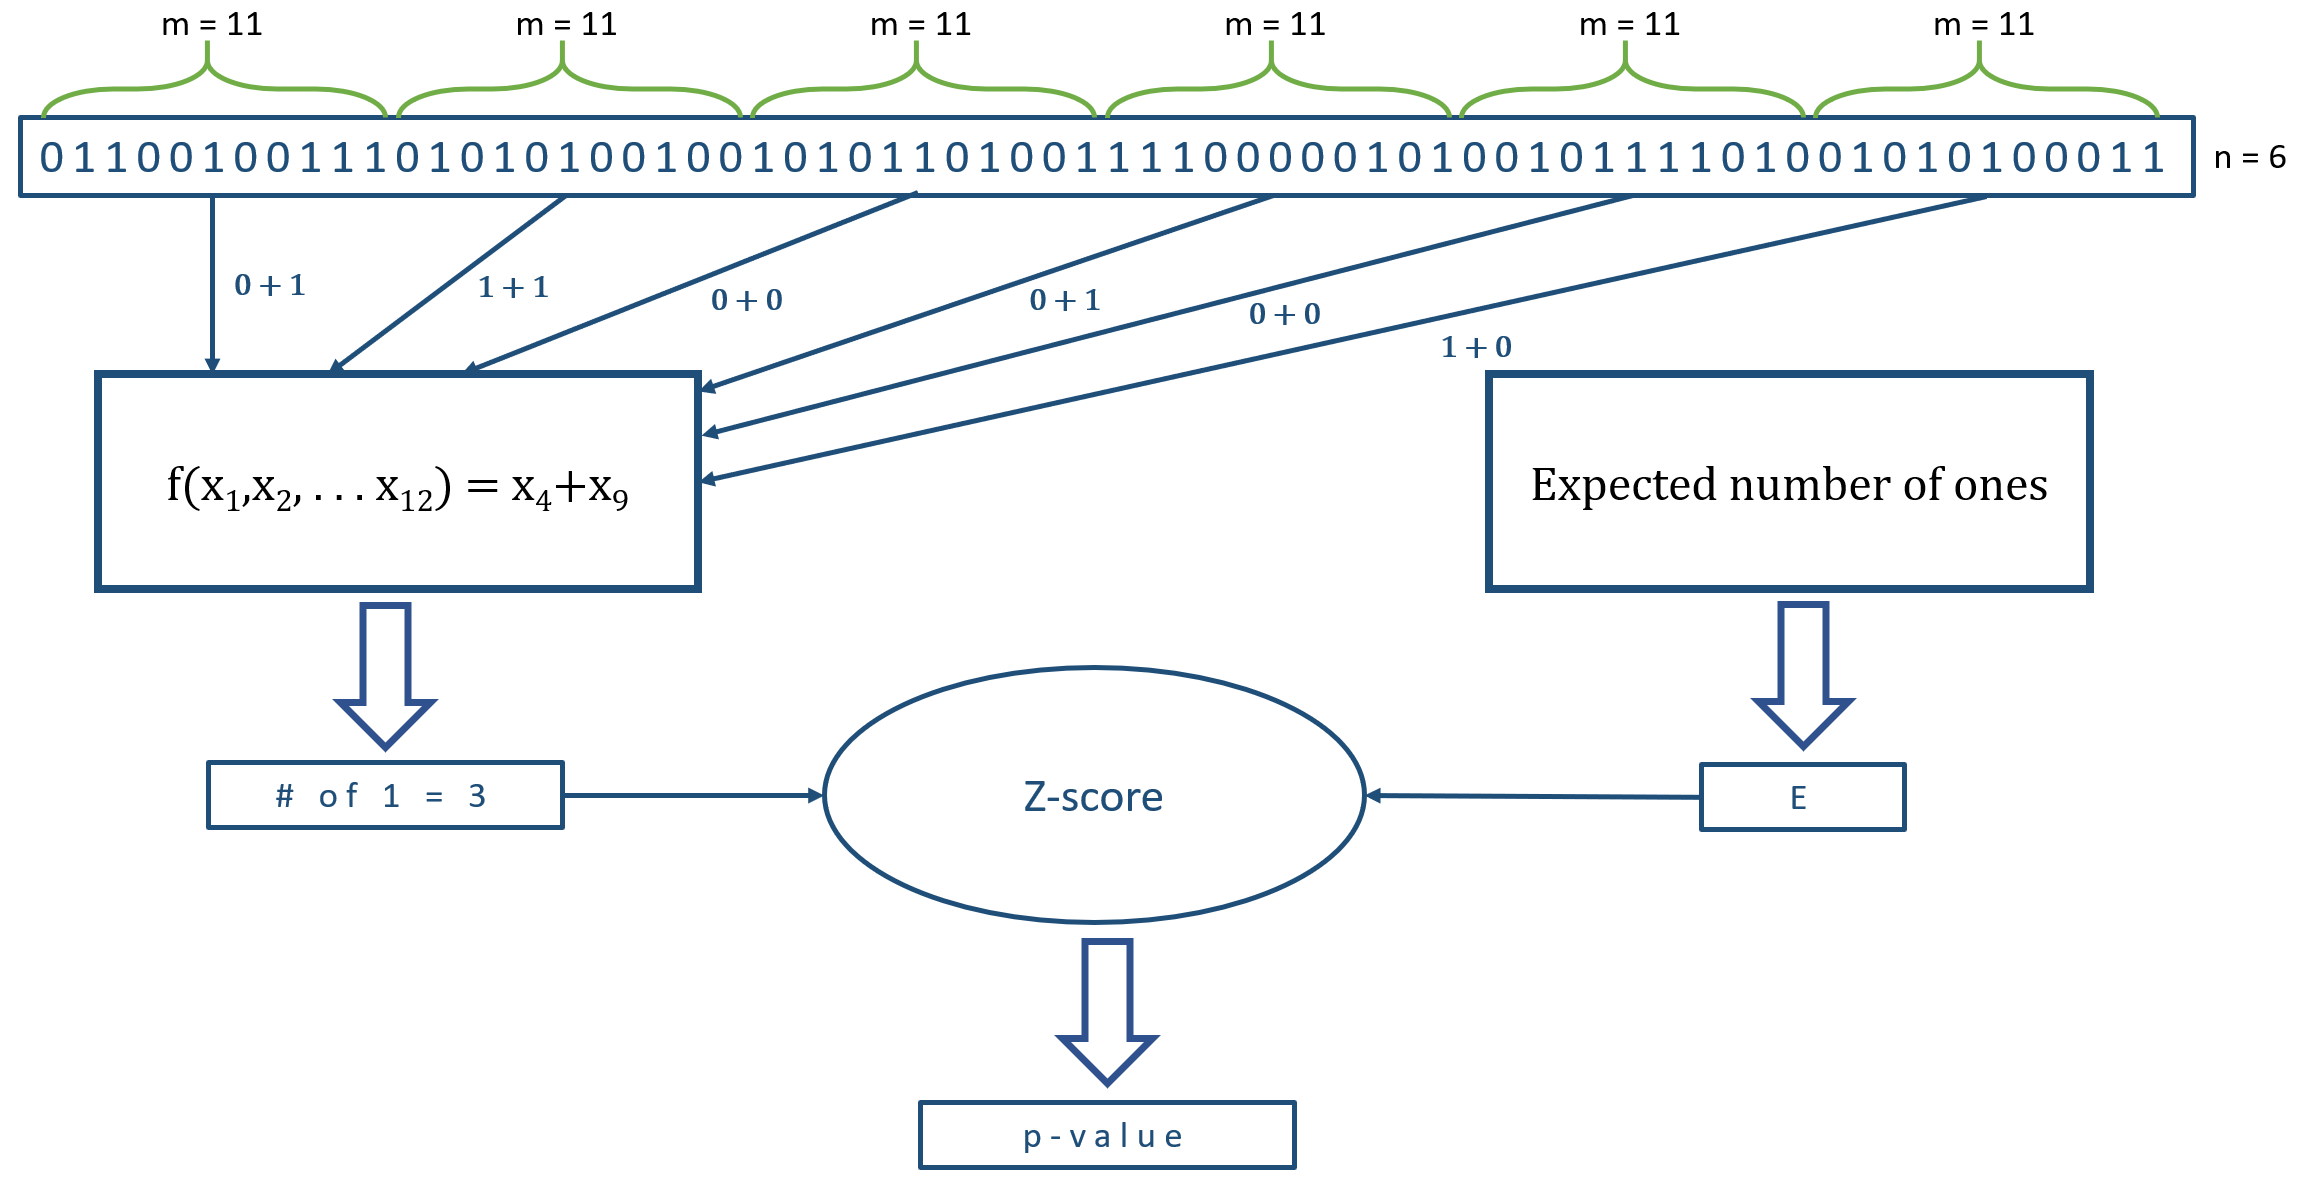
\includegraphics[width=0.8\textwidth]{./images/pictures/bool-test.png}
	\caption{Example of evaluation with BoolTest for sequence of size 66 bits with block size 11 and number of blocks 6. Evaluated Boolean function (distinguisher) is $f(x_1,x_2, . . . x_{11}) = x_4+x_9$.}
	\label{fig:bool-test}
\end{figure}

Construction of distinguisher is based on an assumption that a combination of weaker and simpler Boolean functions may lead to stronger distinguisher. The process starts with brute-force evaluation of all possible Boolean functions of type  $f(x_{1}, x_{2}, \cdot \cdot \cdot, x_{m}) = x_{i}$ for $\forall i \in \{1, 2, \cdot \cdot \cdot, m\}$ with possibility to choose more complex functions in this phase. The complexity of functions is expressed by degree (\textit{deg}) of function, where \textit{deg} represents how many monomials are used. However, the degree cannot be too high as it is necessary to brute-force all possible functions. The number of all combination can be denoted by binomial coefficient ${m}\choose{deg}$. The second phase captures some number (denoted by \textit{t}) of best distinguishers from the first phase, which are then combined with \texttt{XOR} operator. The number of functions combined together is denoted by \textit{k}, hence the number of all combinations can be denoted by binomial coefficient ${t}\choose{k}$. There are two ways how to optimize this approach: by pre-computation of values from the first phase, and by stopping evaluation at any time when reasonably strong distinguisher is found. If no strong distinguisher is found tested data are considered random. \cite{booltest-secrypt2017}

\chapter{Introduction of CryptoStreams tool}
\label{chap:cryptostreams}

CryptoStreams tool is written in C++ language and is developed and maintained by team\footnote{The team of randomness testing involves following people: Radka Cieslarová, Michal Hajas, Dušan Klinec, Matúš Nemec, Jiří Novotný, Ľubomír Obrátil, Marek Sýs, Petr Švenda, Martin Ukrop and others.} at the Centre for Research on Cryptography and Security, Masaryk University~\cite{CryptoStreams}. The tool is used to generate a large amount of output data streams from parametrized cryptographic functions. Each stream is configurable with multiple options including output length, a structure of input plaintext, key, etc. 

\section{History}

An initial implementation of CryptoStreams project was part of tool EACirc~\cite{EACirc} which was a tool for automatic randomness testing based on genetic programming. At that moment it served only as an internal provider of testing data to its testing functionality and was not possible to use it separately outside of this project. We decided to split those two tools to provide flexible utilization with a broader range of tools in addition to EACirc. EACirc-streams project was introduced in 2017 and then in 2018 it was renamed to nowadays name, CryptoStreams.

\section{Idea}

The main idea behind CryptoStreams is an easy production of data from cryptographic primitives which are reduced in complexity, either by limiting the number of rounds or by providing them input with specific randomness properties, such as low Hamming weight, etc. The most significant advantage is that the tool contains a large number of cryptographic primitives such as block ciphers, hash functions, etc. All of them are integrated within a unified interface. CryptoStreams is also useful as an entry point for investigation of newly created cryptographic primitives, as it is built so that the addition of new primitives was as easy as possible. After obtaining data, it is possible to do any investigation over those data. For example, in this thesis, we conduct statistical analysis with seven statistical batteries of tests and also with a tool called BoolTest~\cite{booltest-secrypt2017}. Notice, that addition of new analysis tool requires no additional implementation on the side of CryptoStreams.

\section{Content of CryptoStreams}

In this section, we would like to present deeper details about what this tool provides. The tool currently contains four types of cryptographic primitives: block ciphers, hash functions, stream ciphers, and pseudo-random number generators. \cref{table:all-cryptoprimitives} shows counts of functions of corresponding types. First cryptographic primitives which were added to CryptoStreams were candidates from SHA-3 and eStream competitions. Those additions were done by Ondrej Dubovec~\cite{Dubovec2012thesis} and Matej Prišťák~\cite{Pristak2012thesis} in 2012. Within those theses were added 34 hash functions and 27 stream ciphers. Another addition was done by Martin Ukrop in his master thesis~\cite{Ukrop2016thesis} regarding authenticated encryption systems from CAESAR competition~\cite{caesar-competition}. Well known block ciphers like AES, DES, etc. were added by Karel Kubíček~\cite{Kubicek2017thesis} and Tamás Rózsa~\cite{Rozsa2018thesis} in their theses. The tool also contains a lot of other cryptographic primitives added outside of theses or papers.


\begin{table}[t]
	\centering	
	\begin{tabular}{|c|c|}
		\hline
		\textbf{\large Cryptographic primitive type} &  \textbf{\large Number of functions} \\ \hline
		Block ciphers  & 42 \\ \hline
		Hash functions & 51 \\ \hline  
		Stream ciphers & 27 \\ \hline
		PRNGS 		   & 6  \\ \hline		
	\end{tabular}
	\caption{List of all types of cryptographic primitives contained within CryptoStreams with the corresponding number of functions.}
	\label{table:all-cryptoprimitives}
\end{table}

Each output is generated by so-called \textit{streams} which are producers of data. Each call produces a chunk of data with configured size. Retrieving data from \textit{stream} in a loop and storing them, results in a data file with desired binary data. By configuring the size of chunk and number of chunks to save it is possible to set the size of resulting file. CryptoStreams contains the following types of streams.

\begin{description}
	\item[\textit{Streams} outputting data with static structure] which are mostly used as an input \textit{streams} such as plaintext or key. Those might be for example binary zero, binary one \textit{stream} or low Hamming weight stream (small amount of ones), etc. Random streams also belong to this category. \cref{fig:static-stream} shows example of schema of such \textit{stream}.
	
	The list of static streams is following:  \texttt{dummy\_stream, true\_stream, false\_stream, mt19937\_stream, pcg32\_stream, counter, random\_start\_counter, sac, sac\_fixed\_position, sac\_2d\_all\_position} and \texttt{hw\_counter}. 

	
	\begin{figure}[h]
		\centering
		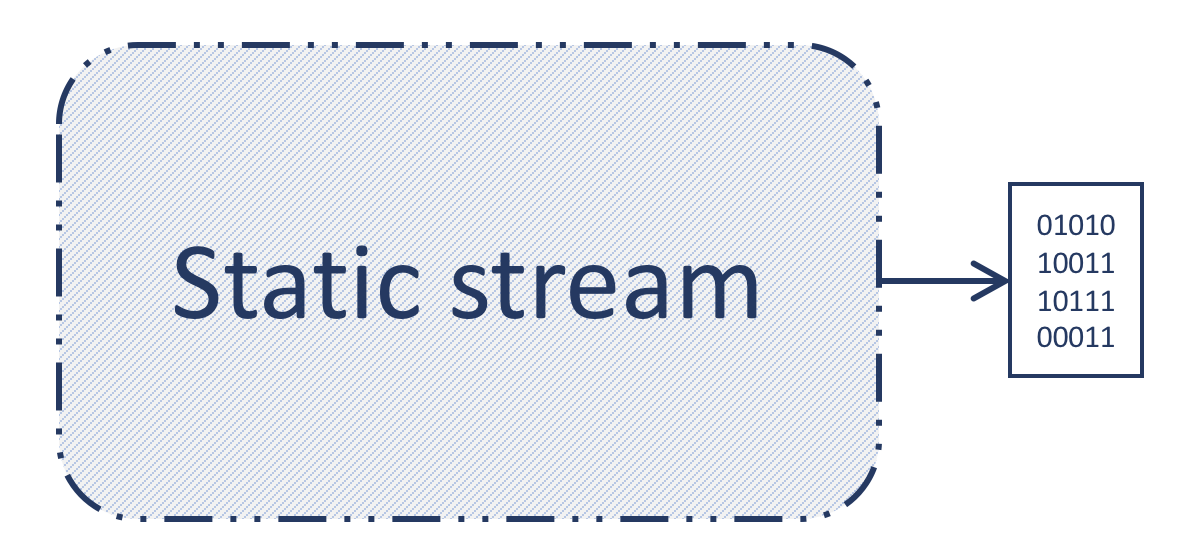
\includegraphics[width=0.5\textwidth]{./images/pictures/static-stream.png}
		\caption{Example of one call of static \textit{stream}.}
		\label{fig:static-stream}
	\end{figure}

	\item[Manipulating \textit{streams}] are configured with one or more input \textit{streams} and manipulate them in a stream-specific way. For example, \textit{repeating stream} is repeating one output specified number of times before generating a new chunk of data from input \textit{stream}. Another example is \textit{tuple stream} that is getting more \textit{streams} as an input and for each call it returns chunk which contains data from each \textit{stream} concatenated together. Schema of this \textit{stream} is shown in \cref{fig:manipulating-stream}. Using tuple stream, it is possible to receive data which consists of plaintexts followed by corresponding ciphertexts.
	
	Currently implemented streams within this category are: \texttt{ single\_value\_stream, repeating\_stream} and \texttt{tuple\_stream}.
	
	\begin{figure}[h]
		\centering
		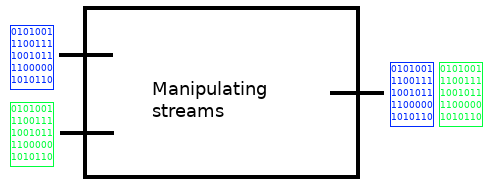
\includegraphics[width=0.7\textwidth]{./images/pictures/manipulating-stream.png}
		\caption{Example of one call from manipulating \textit{stream}, specifically \textit{tuple stream}. }
		\label{fig:manipulating-stream}
	\end{figure}
	
	\item[\textit{Streams} based on round-reduced cryptographic primitives.] Besides the round limitation it is also possible to configure them with various types of plaintext, key and initialization vectors inputs. \cref{fig:crypto-stream} shows a scheme of such stream which uses block cipher. The scheme may be different for other cryptographic primitives, for example, hash functions do not need key or iv as an input.
	
	Project contains 3 types of cryptoprimitves: \texttt{block\_ciphers, stream\_ciphers} and \texttt{hash\_functions}. Number of functions wihitn corresponding category is shown in \cref{table:all-cryptoprimitives}.
	
	\begin{figure}[h]
		\centering
		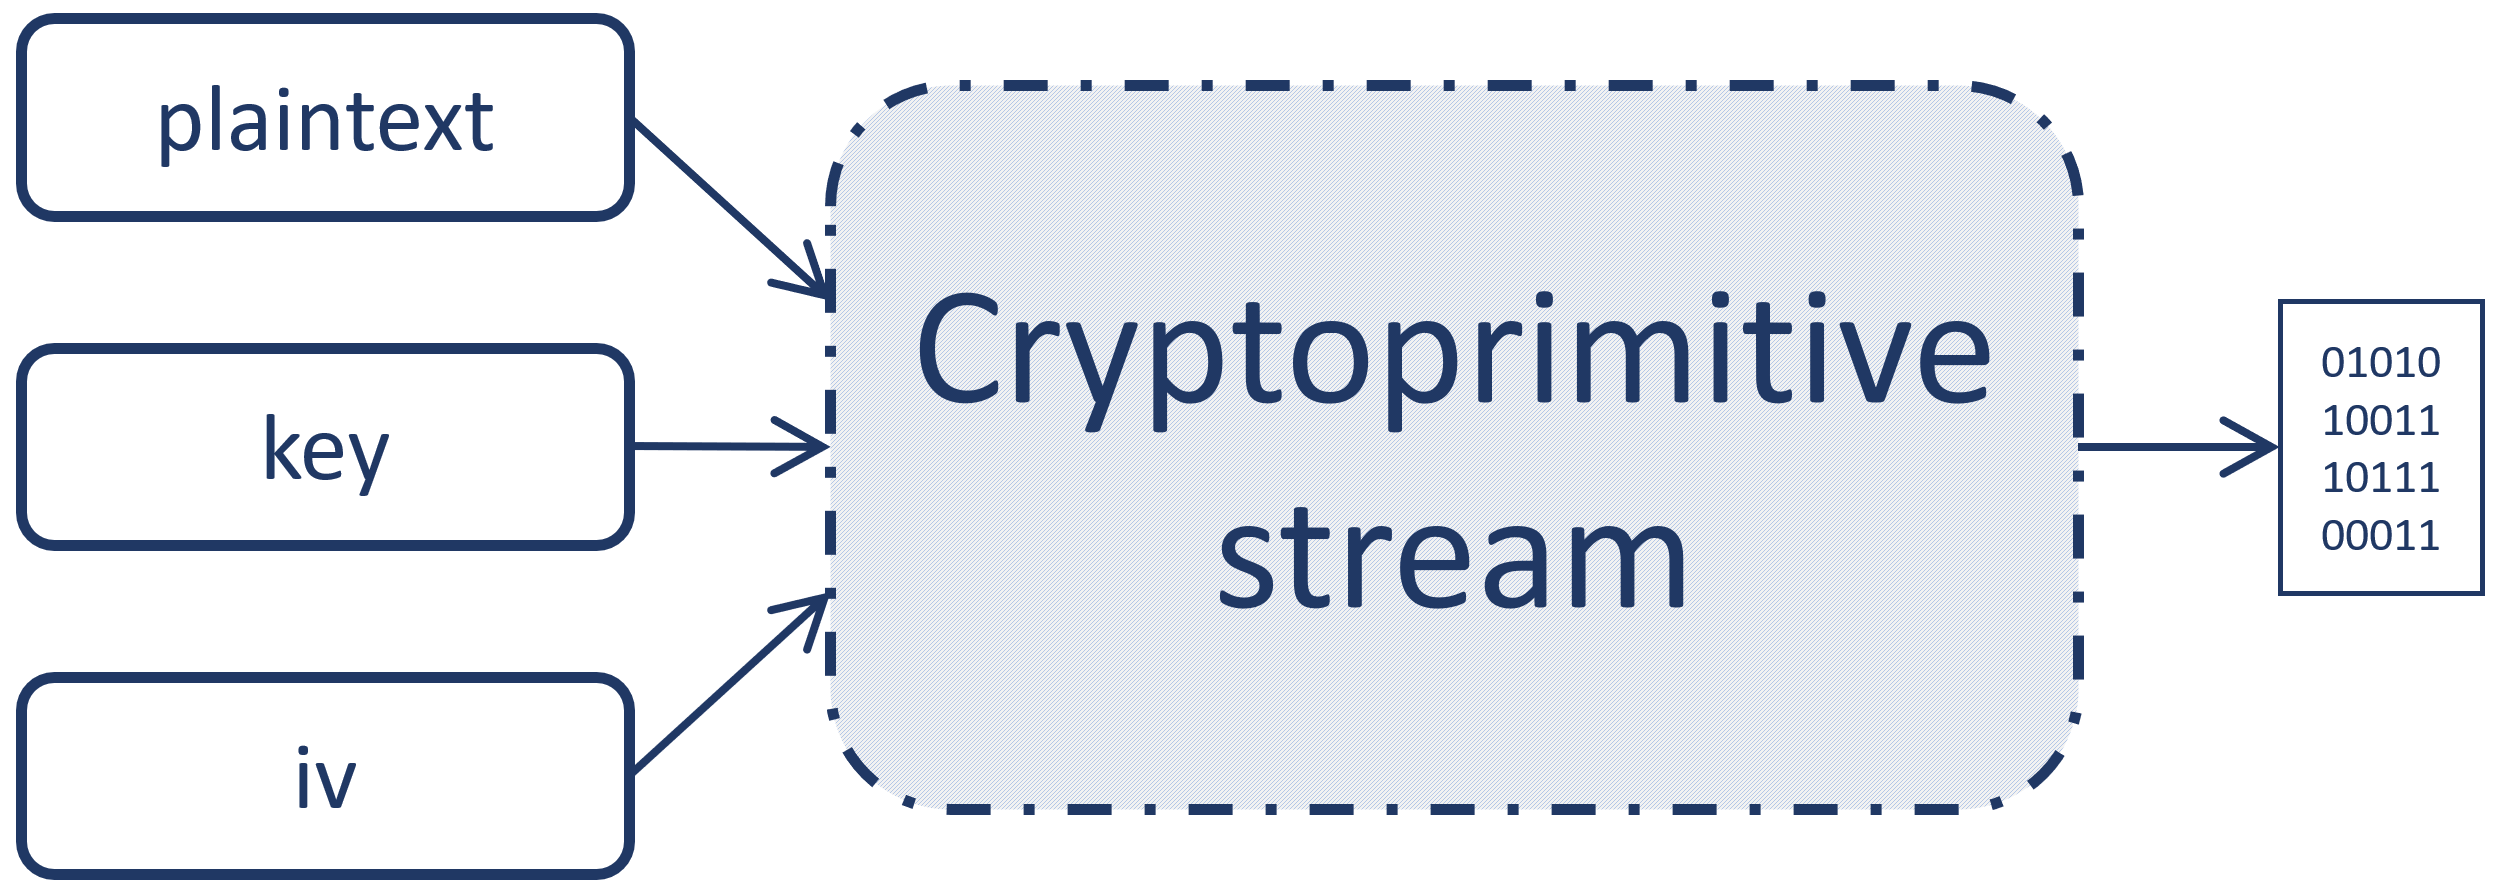
\includegraphics[width=0.7\textwidth]{./images/pictures/cryptoprimitive-stream.png}
		\caption{Example of one call of cryptographic primitive \textit{stream}, where used function is a block cipher.}
		\label{fig:crypto-stream}
	\end{figure}
	
	\item[\textit{Streams} based on pseudo-random number generators.] Those \textit{streams} are introduced as part of this thesis. It is not possible to round-reduce those types of generators; this means the only way how to weaken those generators are to provide them seed with specific randomness properties for example with low Hamming weight. As \cref{fig:prng-streams} shows those \textit{streams} are seeded in the beginning and then provide infinitely many output chunks. It is also possible to reseed generator after some specified number of \textit{chunks} generated. 
	
	All functions within this category are presented in \cref{sec:added_pseudo_random_generators}.
	
	\begin{figure}[h]
		\centering
		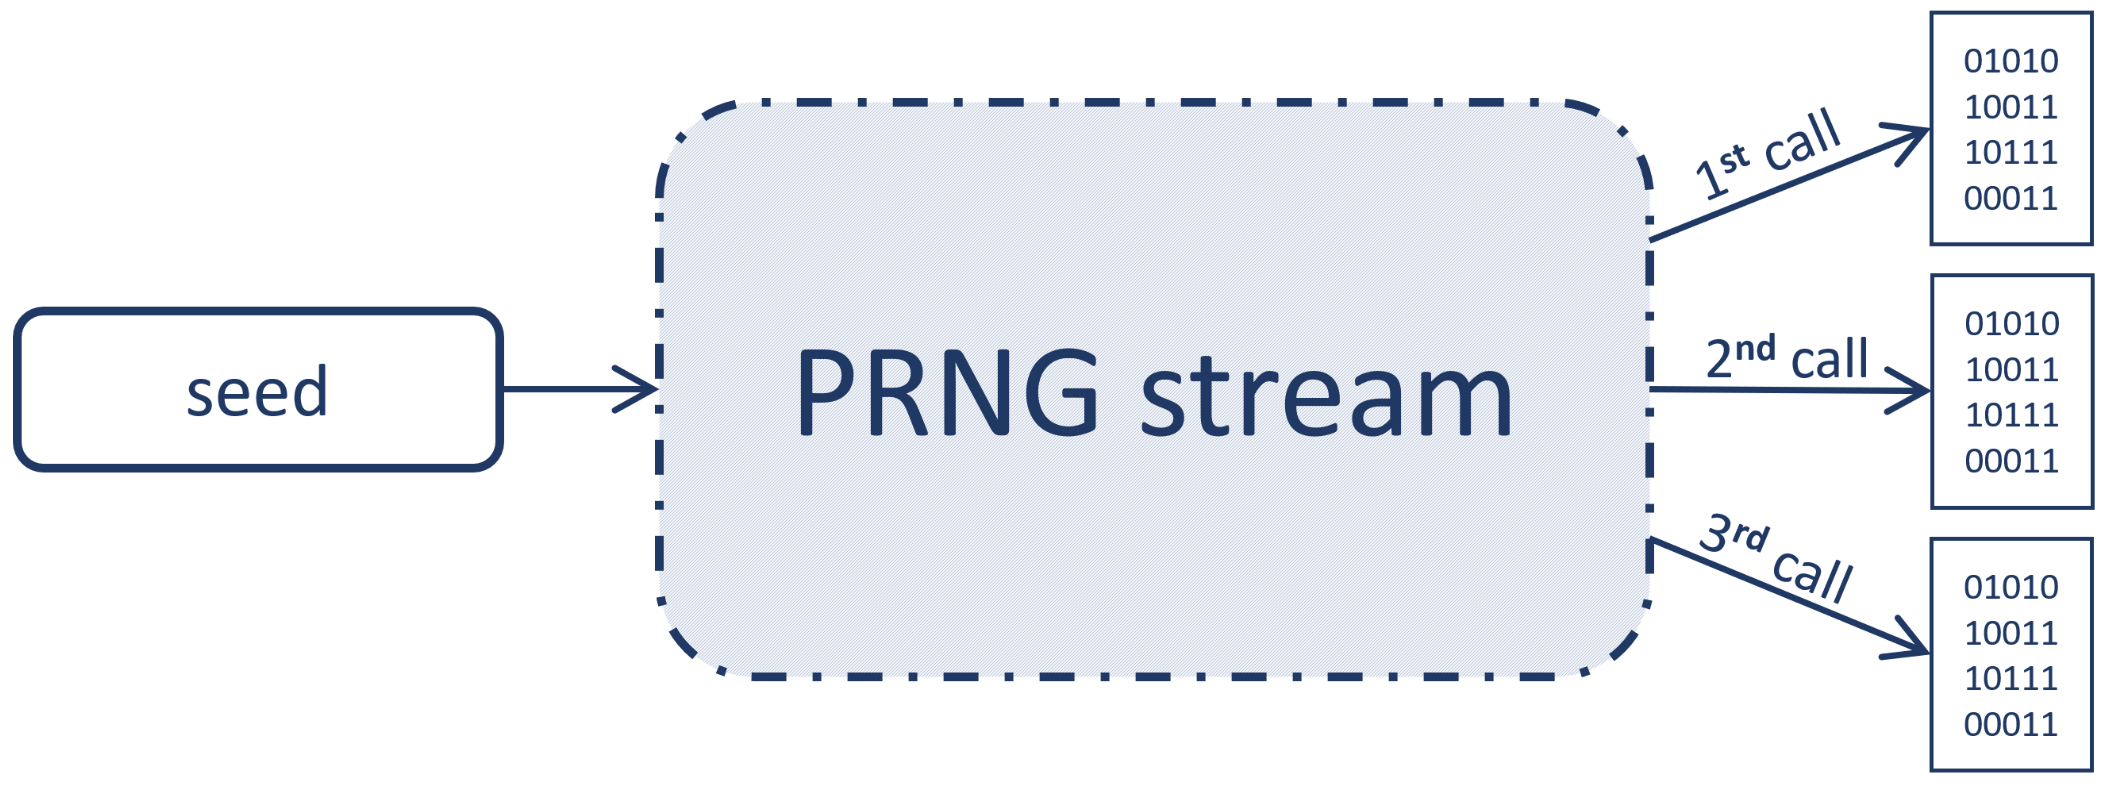
\includegraphics[width=0.7\textwidth]{./images/pictures/prng-stream.png}
		\caption{Example of three calls for a new chunk with same seed from pseudo-random generator \textit{stream}.}
		\label{fig:prng-streams}
	\end{figure}
	
\end{description}

Notice that all inputs are in the form of another \textit{stream}. Receiving \textit{stream} is deciding how much data and when will use from \textit{streams} on its input. For example, if receiving \textit{stream} is a cryptographic primitive type which requests new plaintext for each chunk (e.g., from input static stream), but the key is random and fixed for the whole generation. See the figure \cref{fig:config-schema} for an example of a scheme of the whole run of CryptoStreams. The middle block is the most important one. It is \textit{cryptographic primitive stream} and on its input it has 3 \textit{static streams}.

\begin{figure}[h]
	\centering
	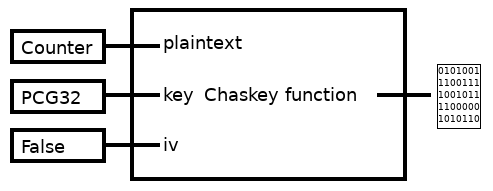
\includegraphics[width=0.7\textwidth]{./images/pictures/config-schema.png}
	\caption{Scheme of CryptoStreams configuration from \cref{fig:json-example}. More information about specific \textit{streams} within this picture can be found in \cref{subsec:configuration} }
	\label{fig:config-schema}
\end{figure}


\subsection{Configuration}
\label{subsec:configuration}

All necessary configuration within one run is achieved using a \texttt{JSON} file. Example of such configuration file can be found in \cref{fig:json-example} which will result in a file of size 8GB, generated from the AES function limited to 5 rounds. Key is generated pseudo-randomly using PCG32~\cite{pcgGen} at the beginning of a run and then used for generation of each output chunk. \textit{Counter stream} is used to generate plaintext blocks. Scheme of this configuration is shown in \cref{fig:config-schema}. 

The whole run of the generator is deterministic as it is using a pseudo-random generator with a specified seed. Experiments are therefore fully replicable using only stored \texttt{JSON} configuration. Notice that resulting file size is derived from \texttt{chunk\_size} in Bytes and \texttt{chunk\_count}. All possible options of configuration of CryptoStreams can be found in project documentation~\cite{CryptoStreams-wiki}.

\begin{figure}[h]
	\centering
	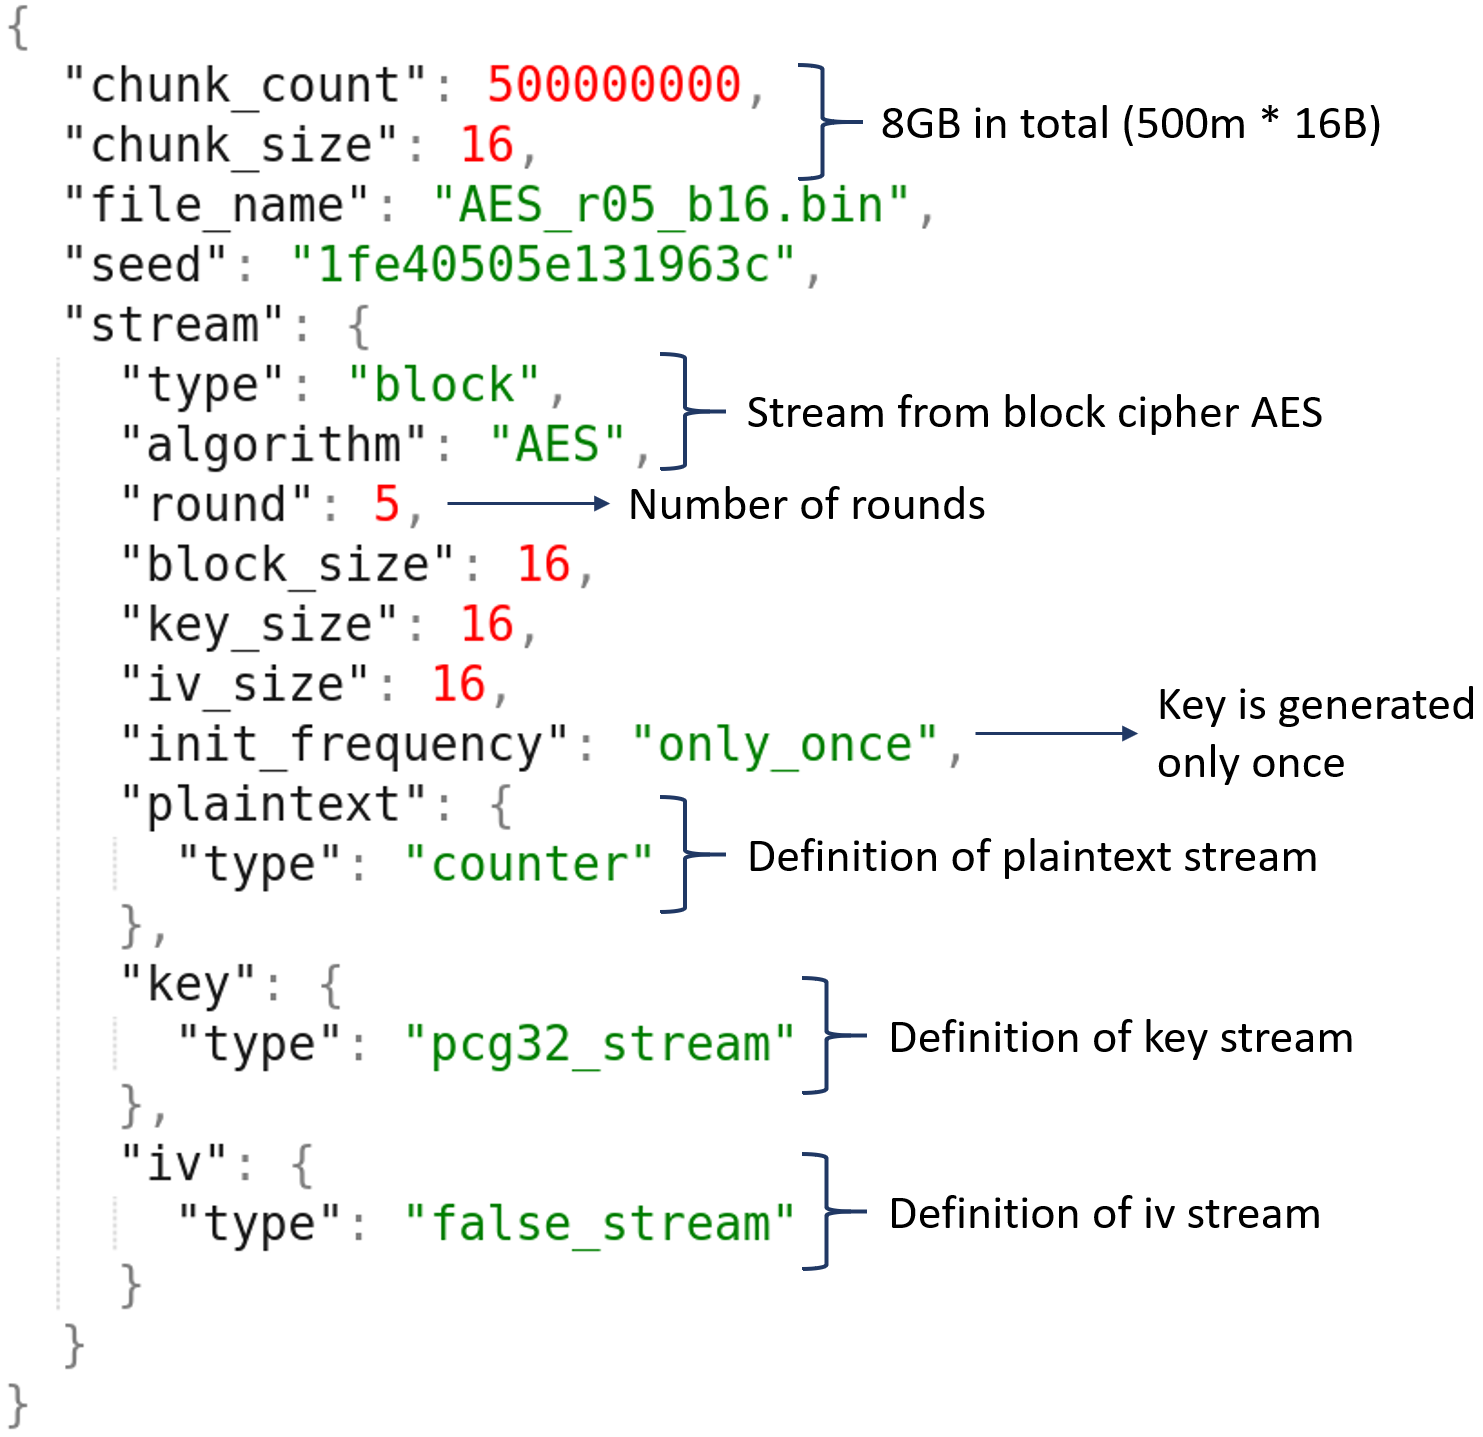
\includegraphics[width=0.7\textwidth]{./images/pictures/config.png}
	\caption{Example of \texttt{JSON} configuration for the tool CryptoStreams.}
	\label{fig:json-example}
\end{figure}


\subsection{Testing of streams}

Our statistical analysis relies on the fact that data which come from CryptoStreams are correct and genuinely come from cryptographic primitives. For that reason, we introduced testsuite which contains a various number of tests per individual \textit{stream}. We have added tests only for most frequently used \textit{streams}. Tests are also required for all newly added \textit{streams}. Results in this thesis are based on \textit{streams} which are tested.

As testing backend we are using Google Test~\footnote{\url{https://github.com/google/googletest}} framework. To ensure all tests are passing for each new change we use continuous integration tool called Travis CI\footnote{\url{https://travis-ci.org}}.

There are two things which are important to test. First one is function itself, source code which is included within CryptoStreams. The other thing is CryptoStreams superstructure which encapsulates all cryptographic primitives and functions into one interface. Each type of \textit{streams} have different testing scenarios.

\begin{description}
	\item[Block ciphers \textit{streams}] are tested with test vectors in both directions, encrypt and decrypt. Also, both mentioned layers are tested. All those tests are testing function only in the full number of rounds as we were not able to find test vectors for round limited version. For lightweight cryptographic primitives based \textit{streams} we also added an \textit{encrypt-decrypt} test, for all supported rounds which is testing whether encryption of plaintext followed by decryption results with inputted plaintext. However, this test does not work for all added functions; the reasons are summarized in \cref{sec:added_lightweight_crypto}. Test coverage is complete for block ciphers with all 42 functions supplied with test vectors.
	
	\item[Hash functions \textit{streams}] are tested with test vectors in the full number of rounds. Both low-level function and CryptoStreams superstructure are included in tests. 29 out of 51 hash functions are covered with tests.
	
	\item[Stream ciphers \textit{streams}] are tested similarly to block ciphers except for encrypt-decrypt test for round reduced versions. From 27 stream ciphers 15 are tested.
	
	\item[Pseudo-random generators \textit{streams}] are hard to test, we have not found any test vectors. Nonetheless, we at least added test for linear generators by implementing an expected succession of numbers in tests and then compare whether we are getting same numbers from generator implementation. Four generators out of six included in CryptoStreams are tested. However, one test is testing only whether the generator is running without checking the correctness of output.
	
	\item[Other \textit{streams},] static or manipulating, are easy to test as we know how exactly should output look like.
	 
\end{description}
\begin{table}[t]
	\centering	
	\begin{tabular}{c|c c c c}
		\textbf{\large Crypto primitive type} &  Block ciphers &  Hash functions &  Stream ciphers &  PRNGS  \\ \hline
		\textbf{\large Tested/All functions} & 42/42	&	29/51		&		15/27	&		4/6	\\
		
	\end{tabular}
	\caption{List of all types of cryptographic primitives with the number of functions covered with tests.}
	\label{table:tested-cryptoprimitives}
\end{table}

\section{Conducted experiments}
\label{sec:conducted-experiments}

The experiments we conducted were based on testing of randomness provided by cryptographic primitives in some extreme scenario. We tested the following scenarios.

\begin{description}
	\item[A specific type of input,] mostly with some lousy randomness properties, is provided to functions (either as a plaintext block ciphers or seed for PRNGs) and statistical analysis is conducted where results are compared with random or other specific inputs. For this thesis, we used the following types of inputs.
	\begin{enumerate}
		\item Counter \textit{stream} is such \textit{stream} in which each chunk is the addition of one to the previous chunk in number representation.
		\item Low Hamming weight \textit{stream} returns outputs with least count of ones it is possible. Starting with all zeroes followed with only binary one on each position, two binary ones, etc.
		\item Strict avalanche criterion is a type of \textit{stream} in which the first chunk is randomly generated, and every next call is just previous chunk with one flipped bit.
	\end{enumerate}
	
	\item[Plaintext-ciphertext stream] produces pairs of input and output to function. With statistical testing performed on such output, it is possible to investigate dependency between plaintext and ciphertext. Since plaintext is part of the resulting sequence it is important to choose data with good randomness properties otherwise it may cause some interference in testing results.
\end{description}

Almost every cryptographic function is build so that it performs a very same sequence of operations defined number of times, mostly in a loop. The number of times sequence should be performed is denoted by term \textit{number of rounds}. For example, AES~\cite{FIPS-197} has a recommended number of rounds 10, 12 or 14 based on key length as you can see in \cref{fig:fips197-rounds}. Each round in AES consists of \textit{SubBytes, ShiftRows, MixColumns, AddRoundKey} operations. The original implementation of AES has different key scheduling phase based on the number of rounds. However, we keep key scheduling in the full number of rounds for all functions in CryptoStreams so that we avoid some undefined behavior based on uninitialized parts of the key.

\begin{figure}[h]
	\centering
	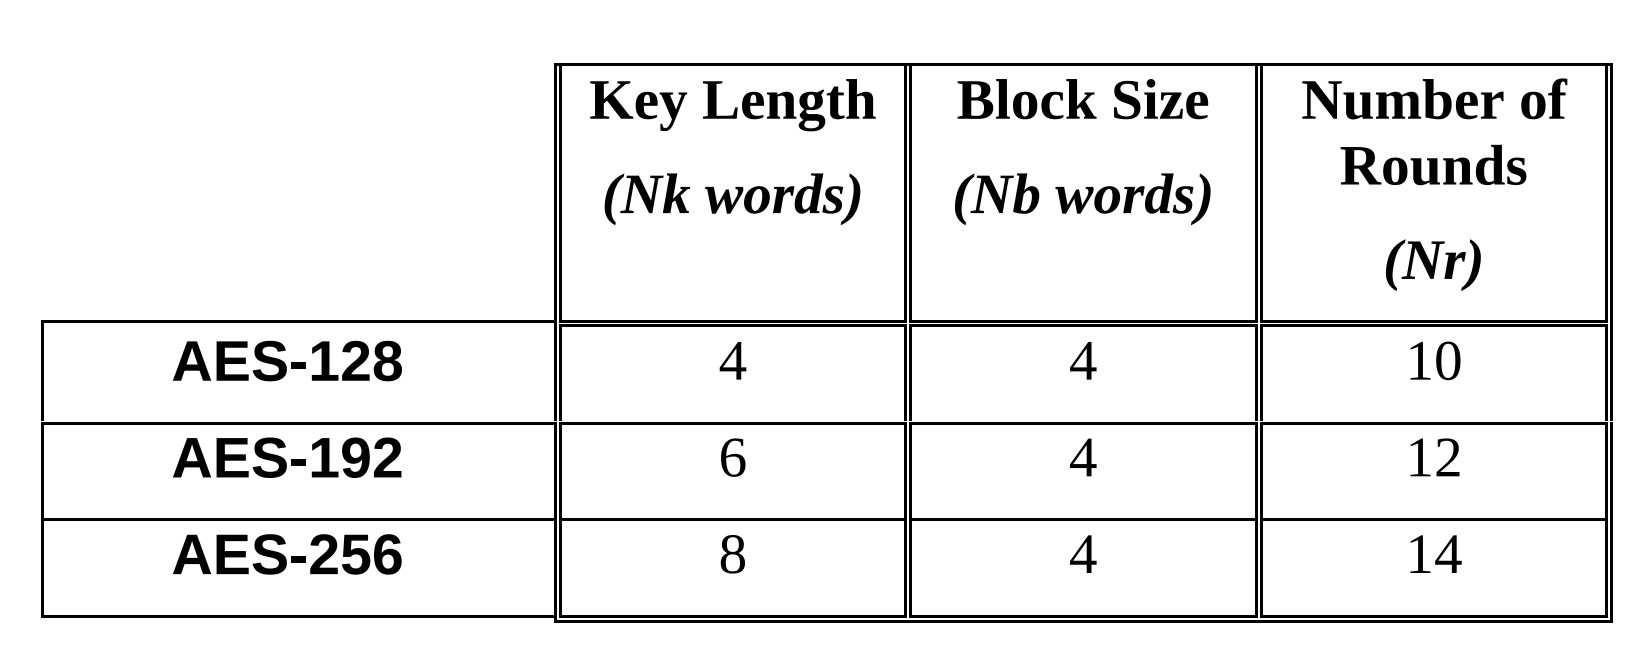
\includegraphics[width=0.4\textwidth]{./images/pictures/FIPS197-Nr-table.png}
	\caption{Table of rounds based on key size which is taken from~\cite{FIPS-197}, word size is 32 bits.}
	\label{fig:fips197-rounds}
\end{figure}

Authors of each cryptographic function specify how many rounds should be used to have reasonable security and performance. This number is called \textit{full number of rounds} and should be determined by conducting all known attacks against function limited to several numbers of rounds. Important indicator during this process is called \textit{security margin}. Security margin denotes the rate between round vulnerable to some cryptanalysis attack and the full number of rounds. For example, at the moment it is not possible to find any practical shortcut attack (any attack which is more efficient than exhaustive key search) for more than six rounds for AES with key length 128 bits. Therefore it is recommended to add four more rounds as a security margin and use AES with ten rounds \cite{daemen1999aes}. Notice that \textit{security margin} is not some general notion for the whole function, instead of that it is just kind of expression of resistance against particular cryptanalysis technique or attack.

In this thesis, the security margin represents the rate between a number of rounds whose output were distinguishable from truly random sequence. The output was obtained from scenarios specified above.

Notice that the round limitation is not available for tested PRNGs. Therefore, for PRNGs, we are testing four different scenarios, where each is using different reseed frequency. First scenario generates whole sequence for one seed, the other three reseeds after 10/100/1000 iterations.  


\subsection{Testing with Randomness testing toolkit}

For running statistical batteries, we are using a tool called randomness testing toolkit (RTT)~\cite{Obratil2017thesis}. It is a project which unifies more software tools for randomness testing under one interface. It provides both graphical interface (GUI) in the form of webpage and command line interface (CLI). CLI is mainly used for submission of a higher number of experiments due to possible automation, for example with python or shell scripts. Also GUI provides webpage form for submission of an experiment, but it is much easier to use CLI for automation. Besides the submission form, the webpage also provides an interpretation of results in a consistent way between all batteries. Three types of assessments OK, SUSPECT and FAIL are assigned to batteries based on the amount of failed test. The results of individual tests within batteries are evaluated with significance level $\alpha = 0.01$.

RTT contains tests from three software tools: {NIST STS}~\cite{nist-sts}, Dieharder~\cite{dieharder} and TestU01~\cite{l2007testu01}. We used all statistical batteries which RTT provides, except for Big Crush from TestU01 because it requires at least 60GB of data per run, which would be too demanding for resources. 

\subsection{Testing with BoolTest}
\label{sec:testing_booltest}

BoolTest has four configurable parameters (all described in \cref{sec:booltest-theory}). The size of the block \textit{m}, the number of monomials in a function in the first phase \textit{deg}, the number of functions captured to second phase \textit{t} and the number of functions combined in second phase \textit{k}. We have chosen the following values within our experiments.

\begin{itemize}
	\item $m = [128, 256, 348, 512]$ 
	\item $deg = [1, 2]$
	\item $t = [128]$
	\item $k = [1, 2]$
\end{itemize}

Those experiments were computed on Metacentrum grid infrastructure. For running jobs on Metacentrum, we used scripts available in BoolTest repository~\footnote{\url{https://github.com/ph4r05/polynomial-distinguishers}} with few changes needed for our scenarios. Using those scripts, it is easy to run new experiments. Scripts are taking care of division of calculations between more machines provided by Metacentrum including generation of configuration for CryptoStreams and BoolTest itself. 

There are also scripts for processing of the results, which generates \texttt{CSV} files with some interpretation of results. The interpretation is based on a comparison of results with reference data generated by AES in the full number of rounds (indistinguishable from truly random data). We conducted 100 reference experiments for each testing scenario, and the average of those is taken as a reference Z-score. Scripts are interpreting results as non-random in case the obtained Z-score is higher than (reference Z-score + 1). However, this does not solve tight values, for example, if obtained Z-score is only slightly higher than (reference Z-score + 1) it does not guarantee the analyzed data are not random. For that reason, we are testing tight cases (obtained Z-score is higher than [reference Z-score + 1] but less than [reference Z-score + 2]) again with the assumption that doubling the data size should not increase the value of Z-score given there is no bias.

\section{Investigated pseudo-random generators}
\label{sec:added_pseudo_random_generators}

In this section, we will present all functions which were incorporated to CryptoStreams and then investigated for indistinguishability from the truly random stream.

\subsection{Pure pseudo-random generators}
\label{subsec:pure-generators}

The first part of this thesis is the addition to CryptoStreams and analysis of pure (do not use any cryptographic primitive to generate pseudo-randomness) pseudo-random number generators. It was not possible to round reduce those generators because the implementation does not provide it. Hence we only weakened them with seed with specific randomness properties. This component is quite small as we added together only six generators. The reason why we added such a small amount of generator is that we have not found any source of generators which would offer generators in a way it would be easy to incorporate to CryptoStream.

One of the sources of generators was a TestU01~\cite{l2007testu01} project. It contains a high number of generators, but they offer just implementations without parameters set up. So we needed to find out those parameters ourselves, and it was sometimes difficult to choose correctly. Reasons for difficulties was, for example, selecting parameters so that output was long enough to fill 8 bytes of data, absence of literature for less widely used generators, etc. We have taken over three generators and also included some basic tests. All generators are appropriately described in TestU01 user guide \cite{LEcuyer07testu01}.
\begin{description}
	\item[Linear congruential generator.] Definition of this generator is shown in \cref{formula:lcg}. Chosen parameters are taken from \cite{L-Ecuyer:LCG} and values are $a = 4645906587823291368$, $c = 0$ and $m = 9223372036854775783$. We have chosen as big parameter \textit{m} as possible because the generator is outputting values modulo this parameter, this means values are always less than this number. Since returning value from the generator is always 8 bytes long and the number $ 9223372036854775783 $ have few upper bits binary zeroes, also outputting value will always have those bits binary zero. For that reason, we cut those bits to not have any interference caused by too many zeroes in statistical tests. This is the main reason for adding such a small number of generators in this thesis because it would require too much configuration and testing to be sure the generators are working properly.
	
	\item[Multiple recursive generator.] Another linear generator, which is based on a very similar principle as LCG, with the difference that it combines data from more than one previous run. It is based on following formula.
	
	\begin{equation}
	x_{n} = \left(a_{1} \times x_{\left(n-1\right)} + . . . + a_{k} \times x_{\left(n-k\right)}\right)~~\bmod~~m
	\end{equation}
	
	Where \textit{k, $a_{1} .. a_{k}$ and m} are parameters of the generator hardcoded in CryptoStreams, $X_{n-l}$ is an output of a run $n-l$ where $n$ is current run and $l$ is a number between $1$ and $k$. The seed represents initial values of $X_{1}$ to $X_{k}$.
	
	 Chosen parameters are following: $ k = 2 $, $ a_{1} = 2975962250 $, $ a_{2} = 2909704450 $ and $ m = 9223372036854775783 $ \cite{L_Ecuyer:MRG}. We are cutting upper binary zeroes similarly like in LCG.
	
	\item[Xorshift generator.] The generator is based on \textit{xor} and \textit{shift} operations~\cite{RePEc:jss:jstsof:v:008:i14}. We have chosen version which is created by function \texttt{uxorshift\_CreateXorshift13} and requires no additional parameters, more information in \cite{LEcuyer07testu01} on page 50. \\
\end{description}

The second source of pseudo-random number generators is the standard library of C++. Unlike TestU01 it contains generators including parameters. It is less complicated to take over this code as it is enough to use \texttt{include} directive. The only disadvantage of this source is it contains only three pseudo-random generators. List of generators is following.

\begin{description}
	\item[Linear congruential generator~\footnotemark.] The same generator as we have taken over from TestU01. The definition is shown in \cref{formula:lcg}. Used parameters are $a = 48271$, $c = 0$ and $m = 2147483647$. As you can see numbers are much smaller, than those we have chosen for the generator from TestU01. The reason is that this generator outputs only 4 Bytes instead of 8 Bytes. 
\end{description}
	
	\footnotetext{\url{https://en.cppreference.com/w/cpp/numeric/random/linear\_congruential\_engine}}
	
\begin{description}
	\item[Mersenne Twister~\footnotemark.] The generator was developed by Makoto Matsumoto and Takuji Nishimura \cite{Matsumoto:1998:MTE:272991.272995}. However, it does not produce cryptographically secure random numbers \cite{jakobsson2014theory}. 
	
\end{description}

\footnotetext{\url{https://en.cppreference.com/w/cpp/numeric/random/mersenne\_twister\_engine}}

\begin{description}

	\item[Substract with carry~\footnotemark.] This type of generator was introduced by George Marsaglia and Arif Zaman \cite{marsaglia1991}. The definition is following:
	
	\begin{equation}
	x_{n} = \left(x_{n-S} - x_{n-R} - cy(n-1)\right)~~\bmod~~M
	\end{equation}
	Where 
	
	\begin{equation}
	cy(n) = \begin{cases}
	1, & \text{if } x_{n-S} - x_{n-R} - cy(n-1) < 0\\
	0, & \text{otherwise}
	\end{cases}
	\end{equation}
	and \textit{S,R} are parameters hardcoded in CryptoStreams. $x_{k}$ represents $k$-th output of the generator. The seed represents initial values of $x_{1}$ to $x_{k}$ where $k = max{R, S}$.
	
\end{description}

\footnotetext{\url{https://en.cppreference.com/w/cpp/numeric/random/subtract\_with\_carry_engine}}

Specifications details like seed size and output size are shown in \cref{table:prng-properties}


\begin{table}[t]
	\centering
	\begin{tabular}{|c|c|c|}
		\hline
		\textbf{\large PRNG} & \textbf{\large Seed size} & \textbf{\large Output size} \\ \hline \hline
		
		 \textbf{\large TU01 LCG} & 7B & 7B \\ \hline
		 \textbf{\large TU01 MRG} & 14B & 7B \\ \hline
		 \textbf{\large TU01 Xorshift} & 32B & 7B \\ \hline \hline
		 \textbf{\large STD LCG} & 4B & 4B \\ \hline
		 \textbf{\large STD SWC} & 4B & 4B \\ \hline
		 \textbf{\large STD MT} & 4B & 4B \\ \hline
		
	\end{tabular}
	\caption{List of all investigated functions, where sizes are given in Bytes. Including information whether encrypt decrypt test passed.}
	\label{table:prng-properties}
\end{table}


\subsection{Generators based on lightweight cryptographic primitives}
\label{sec:added_lightweight_crypto}

The other part contains block ciphers taken over from project FELICS~\cite{dinu2015felics} developed by Daniel Dinu and his group at the University of Luxembourg. This project is conducting a performance analysis of lightweight functions that are intended for embedded devices. We have taken over only the C++ implementation of functions, as we were not interested in implementations optimized for other architectures. We needed to implement round reduction of functions ourselves as the project contained only full round implementation. However, provision of round reduction was mostly straightforward as functions were prepared with round reduction in mind and we only needed to replace constant in a loop with a variable which is configurable from CryptoStreams. 

Besides the main loop, functions mostly contain also key scheduling, initial and final part. Key scheduling is taking care of the creation of round keys based on a provided key. Initial and final part serves for initialization and finalization of the process. We do not round-reduce any of those parts as we wanted to avoid some memory problems like uninitialized or wrongly cleaned memory.

\cref{table:list-of-investigated functions} contains all investigated functions including some basic information about them. Our intention was also adding two test scenarios, for testing correctness of implementation, for each added function. 

The first scenario is testing all functions with test vectors in full number of rounds. Test vectors were taken over from project FELICS. 

The second test scenario is verifying the expected functionality of round-reduction by doing encryption followed by decryption (Encrypt-Decrypt test) for all rounds provided by tested function. This test is not passing for 6 functions out of 19 (failing marked with \textit{\xmark} in last column in \cref{table:list-of-investigated functions}). The possible explanation of failure is missing round-reduction of key scheduling, which we intentionally do not perform. Despite the failure of the test we observed expected behavior concerning detectable bias by statistical testing -- more rounds results in less bias.

\begin{table}[t]
	\centering
	\begin{tabular}{c|c c c c}
		\textbf{\large Function} & \textbf{\large Round} & \textbf{\large Block size} & \textbf{\large Key size} & \textbf{\large Encrypt-Decrypt test}\\ \hline
		Chaskey~\cite{cryptoeprint:2014:386}				& 16	& 16	& 16	& \cmark	\\ \hline
		Fantomas~\cite{grosso2014ls}						& 12	& 16	& 16	& \cmark 	\\ \hline
		HIGHT~\cite{10.1007/11894063_4}						& 32	& 8		& 16	& \xmark 	\\ \hline
		LBlock~\cite{10.1007/978-3-642-21554-4_19}			& 32	& 8		& 10	& \xmark \\ \hline
		LEA~\cite{Hong2013LEAA1}							& 24	& 16	& 16	& \xmark \\ \hline
		LED~\cite{Guo:2011:LBC:2044928.2044958}				& 48	& 8		& 10	& \cmark \\ \hline
		Piccolo~\cite{10.1007/978-3-642-23951-9_23}			& 25	& 8		& 10	& \cmark \\ \hline
		PRIDE~\cite{10.1007/978-3-662-44371-2_4}			& 20	& 8		& 16	& \xmark  \\ \hline
		PRINCE~\cite{10.1007/978-3-642-34961-4_14}			& 12	& 8		& 16	& \cmark \\ \hline
		RC5-20~\cite{10.1007/3-540-60590-8_7}				& 20	& 8		& 10	& \cmark \\ \hline
		RECTANGLE-K80~\cite{Zhang2015}						& 25	& 8		& 16	& \xmark \\ \hline
		RECTANGLE-K128~\cite{Zhang2015}						& 25	& 8		& 16	& \xmark \\ \hline
		RoadRunneR-K80~\cite{10.1007/978-3-319-29078-2_4}	& 10	& 8		& 10	& \cmark \\ \hline
		RoadRunneR-K128~\cite{10.1007/978-3-319-29078-2_4}	& 12	& 8		& 16	& \cmark \\ \hline
		Robin~\cite{grosso2014ls}							& 16	& 16	& 16	& \cmark \\ \hline
		RobinStar~\cite{grosso2014ls}						& 16	& 16	& 16	& \cmark \\ \hline
		SPARX-B64~\cite{10.1007/978-3-662-53887-6_18}		& 8		& 8		& 16	& \cmark \\ \hline
		SPARX-B128~\cite{10.1007/978-3-662-53887-6_18}		& 8		& 16	& 16	& \cmark \\ \hline
		TWINE~\cite{twine}									& 35	& 8		& 10	& \cmark \\ \hline
		
		
	\end{tabular}
	\caption{List of all investigated functions, where sizes are given in Bytes. Including information whether encrypt decrypt test passed.}
	\label{table:list-of-investigated functions}
\end{table}



\chapter{Results of experiments}
\label{chap:results}

The last chapter is dedicated to the presentation of results obtained from testing outputs from cryptographic primitives for indistinguishability from truly random sequences. Together, we triggered seven statistical batteries of empirical tests of randomness from three various software tools (NIST STS, Dieharder and TestU01). For running those tests, we used tool Randomness Testing Toolkit~\cite{Obratil2017thesis}. The interpretation of results is described in \cref{sec:statistical-tests}.

Another randomness testing tool we used was BoolTest. We ran 16 different configurations and interpreted the results based on the process described in \cref{sec:testing_booltest}.

We investigated outputs from 19 block ciphers and 6 PRNGs. Each cryptographic primitive was inspected within four different testing scenarios described in \cref{sec:conducted-experiments}. Together, each statistical battery analyzed 1584 unique sequences from block ciphers and  96 sequences from PRNGs of size 8GB. With BoolTest, we only analyzed border rounds (rounds on edge between distinguishable and indistinguishable from truly random sequence according to results from empirical tests of randomness). Therefore the number of examined sequences is smaller.

We present the obtained results from different point of views. Firstly we demonstrate security margins for tested block ciphers in \cref{sec:security-margins-results} with respect to indistinguishability of output from a truly random sequence. In \cref{sec:general results for batteries} we compare the highest results achieved for each testing scenario and tool. A comparison of individual batteries within TestU01 is presented in \cref{sec:results of testu01}. In \cref{sec:results of booltest} we present comparison of configurations for BoolTest, and at the end, we show the dependency between the frequency of reseeding of PRNGs and randomness properties of output in \cref{sec:results for PRNGs}.
 
\section{Security margins of tested block functions}
\label{sec:security-margins-results}

\begin{figure}[h]
	\centering
	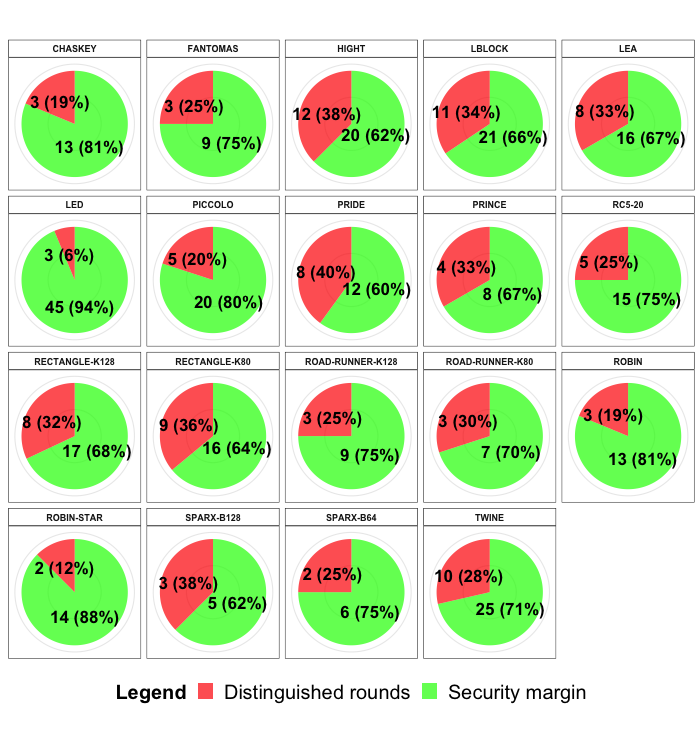
\includegraphics[width=0.9\textwidth]{./images/pictures/security_margins.png}
	\caption{Number of distinguished rounds for corresponding cipher is shown in red. Security margin in green.}
	\label{fig:security_margins}
\end{figure}

Security margin is an important number. In case it is small, with respect to some attack, it signifies that a slight improvement of the attack in future, may result with a successful attack against the full number of rounds of function. Notice that the security margin for other cryptanalysis or attack may be different. 

For PRNGs, we were unable to compute security margin, as they do not have a round reduction. Therefore, in this section, we provide results only for tested lightweight block ciphers. The whole list is shown in \cref{table:list-of-investigated functions}.

\cref{fig:security_margins} shows a pie chart for each tested block cipher. Each pie chart expresses a number of rounds of the corresponding cipher which produce an output which is distinguishable from truly random sequence in red color and the remaining number of rounds, which can be denoted as the security margin, in green color. For example, Chaskey function has the full number of rounds 16, and we were able to distinguish rounds 1, 2 and 3 with at least one of our testing tool. Therefore, the pie chart contains number 3 in red and number 13 in green. The security margin in percents for function Chaskey, with respect to indistinguishability from a truly random sequence, is 13/16 (81\%).

Notice, we are testing only sequences produced by cipher as a black box analysis; we are not doing any steps based on the algorithm of function. Therefore, it is quite likely that for each function, there is an attack focused on this individual cipher (which may take advantage of knowing an algorithm), which performs better than our analysis. Interesting is the comparison between our and their results with respect to the data complexity of an attack. Our analysis has data complexity approximately $2^{33}$ as we are using 8GB of data. For example, Gaëtan Leurent was able to successfully conduct Differential-Linear Cryptanalysis of function Chaskey limited to 7 rounds\cite{cryptoeprint:2015:968} with data complexity $2^{48}$. In three out of four testing scenarios we need ciphertexts only, but in the last scenario (plaintext/ciphertext) we assume plaintext/ciphertext pairs similarly to Differential-Linear Cryptanalysis. However, the most significant difference is in need of human interaction. While for Differential-Linear Cryptanalysis a cryptanalyst is necessary, our attack is almost entirely automated and easily adaptable on a higher number of cryptographic primitives.

We achieved the highest percentage of distinguished rounds for function PRIDE, where we were able to distinguish eight rounds out of 20, which correspond to 40\% of its full number of rounds (security margin is 60\%). Using differential cryptanalysis, Qianqian Yang et al. were able to perform the attack~\cite{pride-attack} against 18 rounds of PRIDE with data complexity $2^{71}$. Therefore, the security margin for this attack is only 2/20 (10\%).

The worst result (lowest number of distinguished rounds) was achieved for function LED with security margin 45/48 (94\%). This function accomplished reasonable resistance also against Differential cryptanalysis. Florian Mendel et al. attacked 24 rounds \cite{led-attack} (security margin 50\%) with complexity $2^{16}$.

\section{Success rate of batteries}
\label{sec:general results for batteries}

\begin{figure}[htbp]
	\centering
	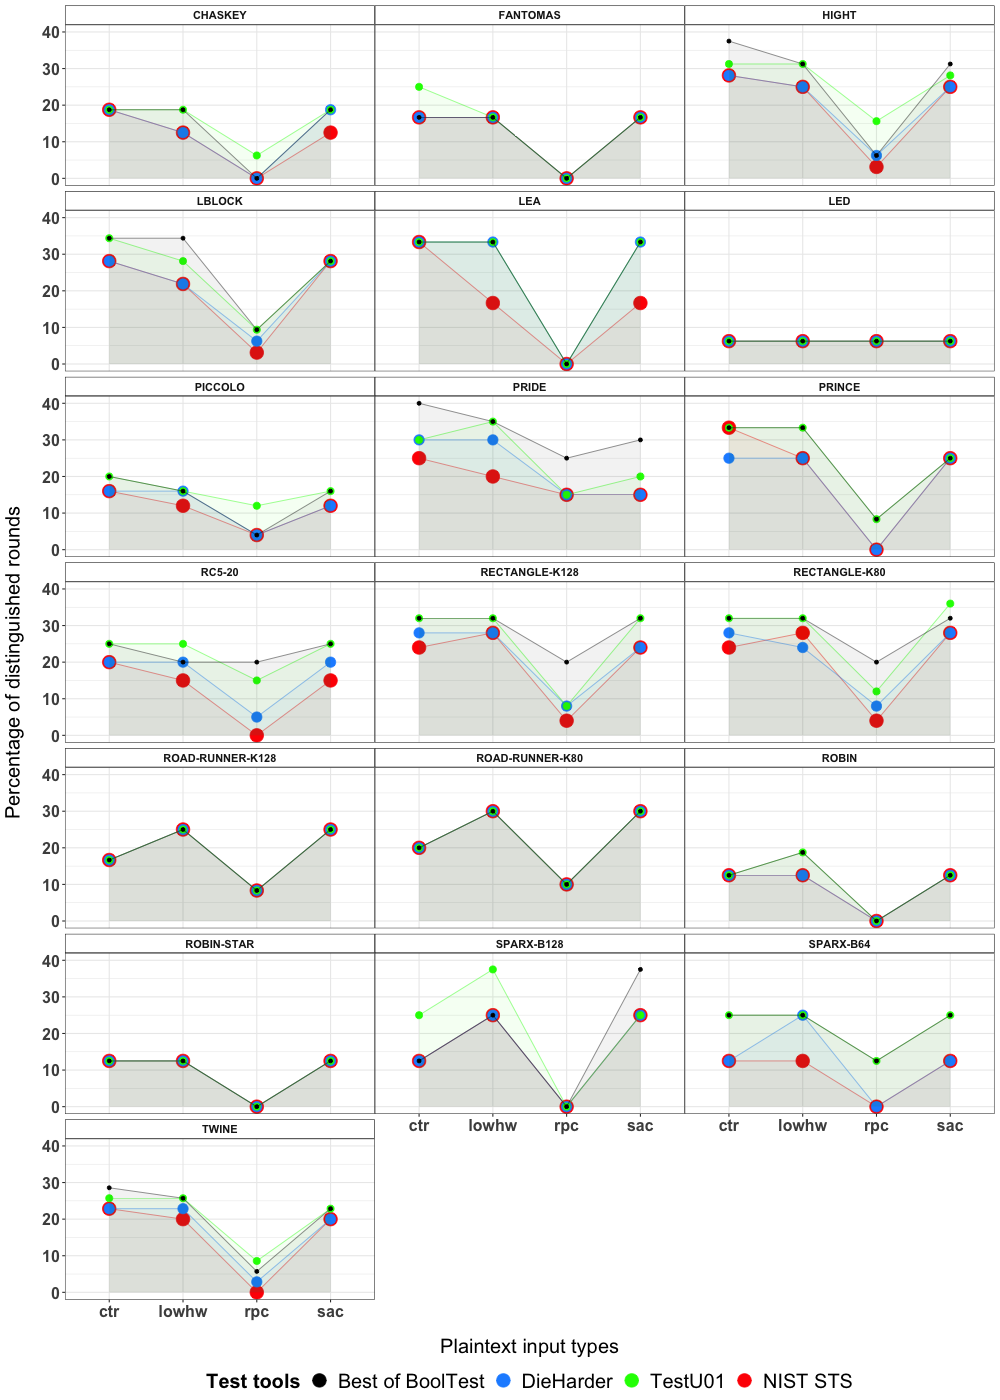
\includegraphics[width=\textwidth]{./images/pictures/batteries_first_part_results.png}
	\caption{Plots for 19 lightweight block ciphers with a percentage of distinguished rounds on Y-axis with respect to plaintext type which is denoted on X-axis. For more information about the interpretation of plots see \cref{sec:general results for batteries}}.
	\label{fig:batteries comparison 1}
\end{figure}

Another view to our result is a comparison of the success, in distinguishing sequences from truly random data, of tools we used. We present results for four software tools (NIST STS, Dieharder, TestU01 and BoolTest). Notice that, in this section, for TestU01 we provide only the highest number of distinguished rounds, which may be achieved by any of the five batteries we triggered, that are part of this tool. For comparison of batteries from TestU01 proceed to \cref{sec:results of testu01}. The same also holds for BoolTest, where the highest result across all 16 configurations is taken into account. \cref{sec:results of booltest} shows differences in achieved results based on changing parameters of BoolTest.

\cref{fig:batteries comparison 1} contains a plot for each tested function. The x-axis corresponds to 4 testing scenarios. Type \textit{ctr} stands for counter \textit{stream}, \textit{lowhw} corresponds to low Hamming weight \textit{stream}, \textit{rpc} to plaintext-ciphertext \textit{stream} and \textit{sac} to strict avalanche criterion \textit{stream}. Y-axis shows a percentage of distinguished rounds for the corresponding function and statistical tool. Colored points express results for tools. Lines are not expressing results (our results are discrete points only), they serve only for better visibility of differences. For example, if there is a green space on top of the plot, it means a battery from TestU01 distinguished the highest number of rounds for corresponding function and input type. As many times we obtained the same results for more batteries, we needed more results in one point to be visible. Therefore, we changed the size of points for each battery; so that if two results overlap, both are visible. This means, if for example NIST STS and Dieharder have the same result, it will be shown as a red point with a smaller blue point inside. 

We can compare results based on two metrics. Either we can compare results for each tool based on its highest result for whole function (together 19 functions), regardless of the testing scenario. Or we can take into account also testing scenario and compare best results for all combinations of function and testing scenario (together 76).

\cref{table:baterries_results} shows a summary of results presented in \cref{fig:batteries comparison 1} comparing both function and sequence types results.

\begin{table}[htbp]
	\centering
	\begin{tabular}{|c|c|c|c|c|}
		\hline
		\multirow{2}{*}{\textbf{\large Testing tool}} & \multicolumn{2}{c|}{\textbf{\large For functions}} & \multicolumn{2}{c|}{\textbf{\large For sequence types}} \\ \cline{2-5}
		& Highest & Exclusively highest & Highest & Exclusively highest \\ \hline
		BoolTest & 17 & 3 & 67 & 11 \\
		Dieharder & 7 & 0 & 33 & 0 \\
		NIST STS & 7 & 0 & 29 & 0 \\
		TestU01 & 16 & 2 &  65 & 9 \\ \hline
		
	\end{tabular}
	\caption{A summary of results for each tool. Results "For functions" are showing the highest results concerning whole functions, while "For sequence types" results are showing the highest results for each sequence type (Function + testing scenario). Exclusively highest stands for a case in which every other tool achieved a worse result. For more details see \cref{fig:batteries comparison 1}.}
	\label{table:baterries_results}
\end{table}

Some observations from test results are following. 

\begin{itemize}
	\item BoolTest distinguished the highest number of rounds exclusively (all other tools were worse) for three functions (HIGHT, PRIDE, and TWINE). TestU01 was solely first in two cases (FANTOMAS and RECTANGLE-K80).
	\item Dieharder and NIST STS were not better for any sequence type than BoolTest or TestU01.
	\item BoolTest performs similarly to TestU01. 
	\item Best combination of tool and input type is BoolTest with counter \textit{stream} and TestU01 with low Hamming weight \textit{stream} which achieved the highest number of rounds for 12 functions.
\end{itemize}

\section{Comparison of TestU01 batteries}
\label{sec:results of testu01}

In previous sections, we compared only highest results from five TestU01 batteries with other testing tools (NIST STS, Dieharder and BoolTest). In this section, we compare only batteries from TestU01 and present which batteries achieved results presented before.

\begin{table}[htbp]
	\centering
	\begin{tabular}{|c|c|c|c|c|}
		\hline
		\multirow{2}{*}{\textbf{\large Testing tool}} & \multicolumn{2}{c|}{\textbf{\large For functions}} & \multicolumn{2}{c|}{\textbf{\large For sequence types}} \\ \cline{2-5}
		& Highest & Exclusively highest & Highest & Exclusively highest \\ \hline
		Alphabit & 8 & 0 & 38 & 1 \\
		Block Alphabit & 14 & 3 & 60 & 7 \\
		Crush & 14 & 1 & 65 & 7 \\
		Rabbit & 12 & 2 &  55 & 2 \\ 
		Small Crush & 7 & 0 &  34 & 1 \\ \hline
		
		
	\end{tabular}
	\caption{A summary of results for each TestU01 battery. Results "For functions" are showing the highest results with respect to whole functions, while "For sequence types" results are showing the highest results for each sequence type (Function + testing scenario). Exclusively highest stands for a case in which every other tool achieved a worse result. For more details see \cref{fig:testu01_all}.}
	\label{table:testu01_summary_results}
\end{table}

\cref{table:testu01_summary_results} shows a summary of the highest results for both, functions and sequence types, achieved by TestU01 batteries. The full list of results for each battery and function is shown in \cref{fig:testu01_all}.

\begin{figure}[htp]
	\centering
	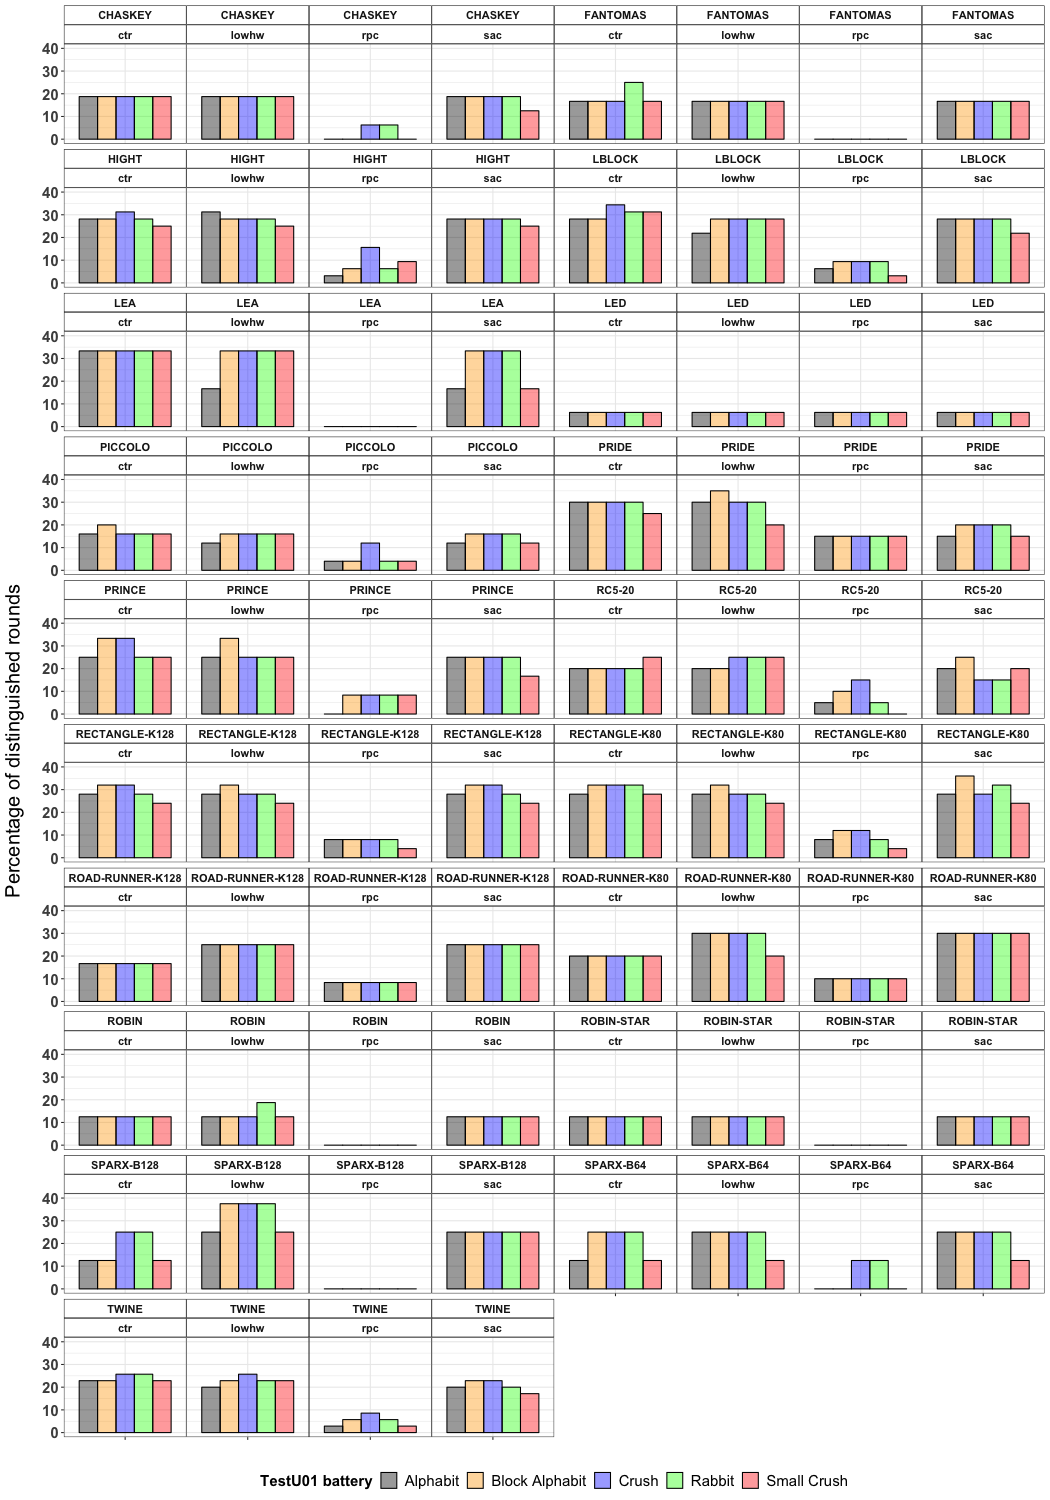
\includegraphics[width=\textwidth]{./images/pictures/testu01_comparison.png}
	\caption{Plots comparing the results for each TestU01 battery. Y-axis shows percentage of distinguished rounds. Each unit show results for a function with a testing scenario for 5 batteries denoted by colored bars. }
	\label{fig:testu01_all}
\end{figure}

Best performing batteries from TestU01 were Crush and Block Alphabit. Block Alphabit distinguished three functions exclusively (PICCOLO, PRIDE, RECTANGLE-K80) while Crush only function LBLOCK. They distinguished an equal number of rounds for 57 sequence types. Crush was better in 12 cases, while Block Alphabit in 7. Notice that from our results, it is not possible to say that Block Alphabit or Crush is the best battery and when testing any cryptographic primitive you can avoid others. However, for testing lightweight block ciphers those two batteries seem to perform better than others.

\section{Comparison of BoolTest configurations}
\label{sec:results of booltest}

Similarly to the TestU01 comparison, in this section, we present a comparison of results achieved by BoolTest. We are showing how changing an individual parameter affects the outcome. We were running BoolTest in 16 different configurations by setting three parameters; all combinations are presented in \cref{sec:testing_booltest}. The meaning of each parameter is described in \cref{sec:booltest-theory}.

Our observations are based on the same principle as in previous sections. We present two types of comparison: the highest result for the whole function and sequence type (function and testing scenario). \cref{table:booltest_summary_results} summarizes results with respect to each configuration, where we show the number of cases in which configurations with a fixed parameter achieved a higher or same result as other options for this parameter. The full results are shown in \cref{fig:bool_test_block} and \cref{fig:bool_test_other}.

\begin{table}[htbp]
	\centering
	\begin{tabular}{|c|c|c|c|c|c|}
		\hline
		\multicolumn{2}{|c|}{\multirow{2}{*}{\textbf{\large Configuration}}} & \multicolumn{2}{c|}{\textbf{\large For functions}} & \multicolumn{2}{c|}{\textbf{\large For sequence types}} \\ \cline{3-6}
		\multicolumn{2}{|c|}{} & Highest & Exclusively highest & Highest & Exclusively highest \\ \hline \hline
		\multirow{4}{*}{\rotatebox[origin=c]{75}{\textbf{Block size}}} 
		& 128 & 16 & 0 & 67 & 6 \\
		& 256 & 18 & 2 & 68 & 2 \\
		& 384 & 14 & 0 & 61 & 0 \\
		& 512 & 15 & 1 &  60 & 0 \\ \hline \hline
		\multirow{2}{*}{\textit{\rotatebox[origin=c]{75}{\textbf{deg}}}} 
		& 1 & 18 & 3 & 68  & 3 \\ 
		& 2 & 16 & 1 & 73 & 8 \\ \hline \hline
		\multirow{2}{*}{\rotatebox[origin=c]{75}{\textbf{\textit{k}}}} 
		& 1 & 17 & 3 & 65 & 3 \\ 
		& 2 & 16 & 2 & 73 & 11 \\ \hline 
		
	\end{tabular}
	\caption{A summary of results for BoolTest based on changing its parameters. The comparison principle is the same as in \cref{table:baterries_results}, with the difference that we are not comparing results across configuration parameters. Result for \textit{deg} is exclusively highest if it is higher than second option. Highest are also those cases when results are same for both. For more details see \cref{fig:bool_test_block} and \cref{fig:bool_test_other}.}
	\label{table:booltest_summary_results}
\end{table}

The results across BoolTest configurations looks more balanced than those comparing different software tools. Taking into account the block size parameter only, lower sizes (128 and 256) seems to perform slightly better, as they distinguished the highest round for more sequence types. However, in some cases, especially for size 128 and strict avalanche criterion input \textit{stream} the number of distinguished rounds dropped to 0 (CHASKEY, FANTOMAS, etc.).

\begin{figure}[htp]
	\centering
	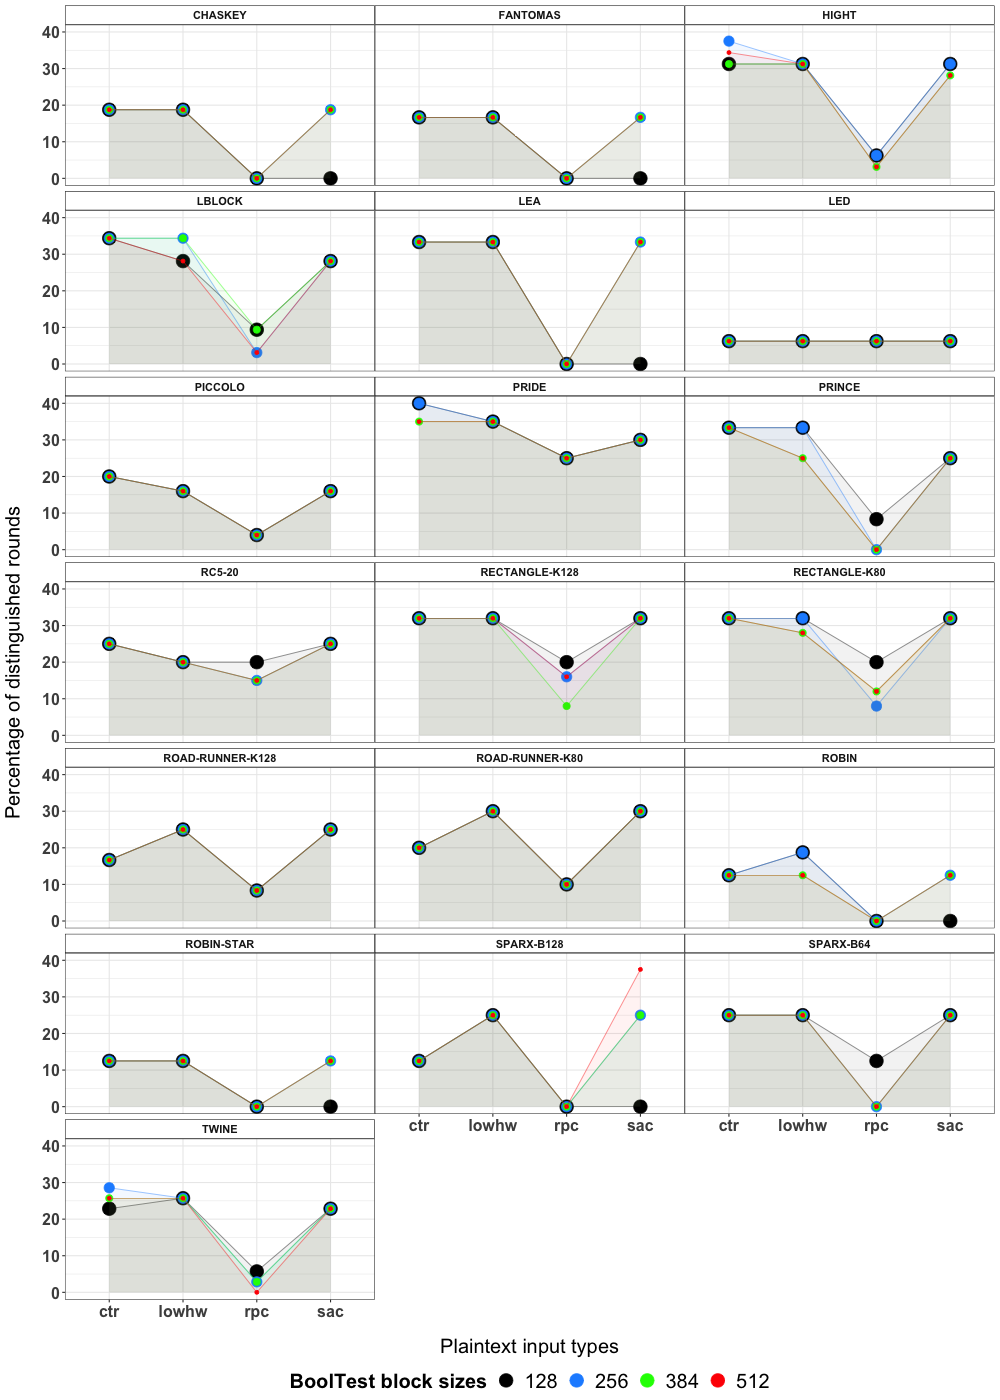
\includegraphics[width=\textwidth]{./images/pictures/bool_test_block_size_comparison.png}
	\caption{Comparison of results with respect to configuration of block size of BoolTest. Y-axis shows percentage of distinguished rounds for testing scenario denoted by x-axis. Each colored point represents highest rounds which was distinguished by BoolTest with corresponding block size, for any combination of \textit{deg} and \textit{k} parameter.}
	\label{fig:bool_test_block}
\end{figure}

\begin{figure}[htp]
	\centering
	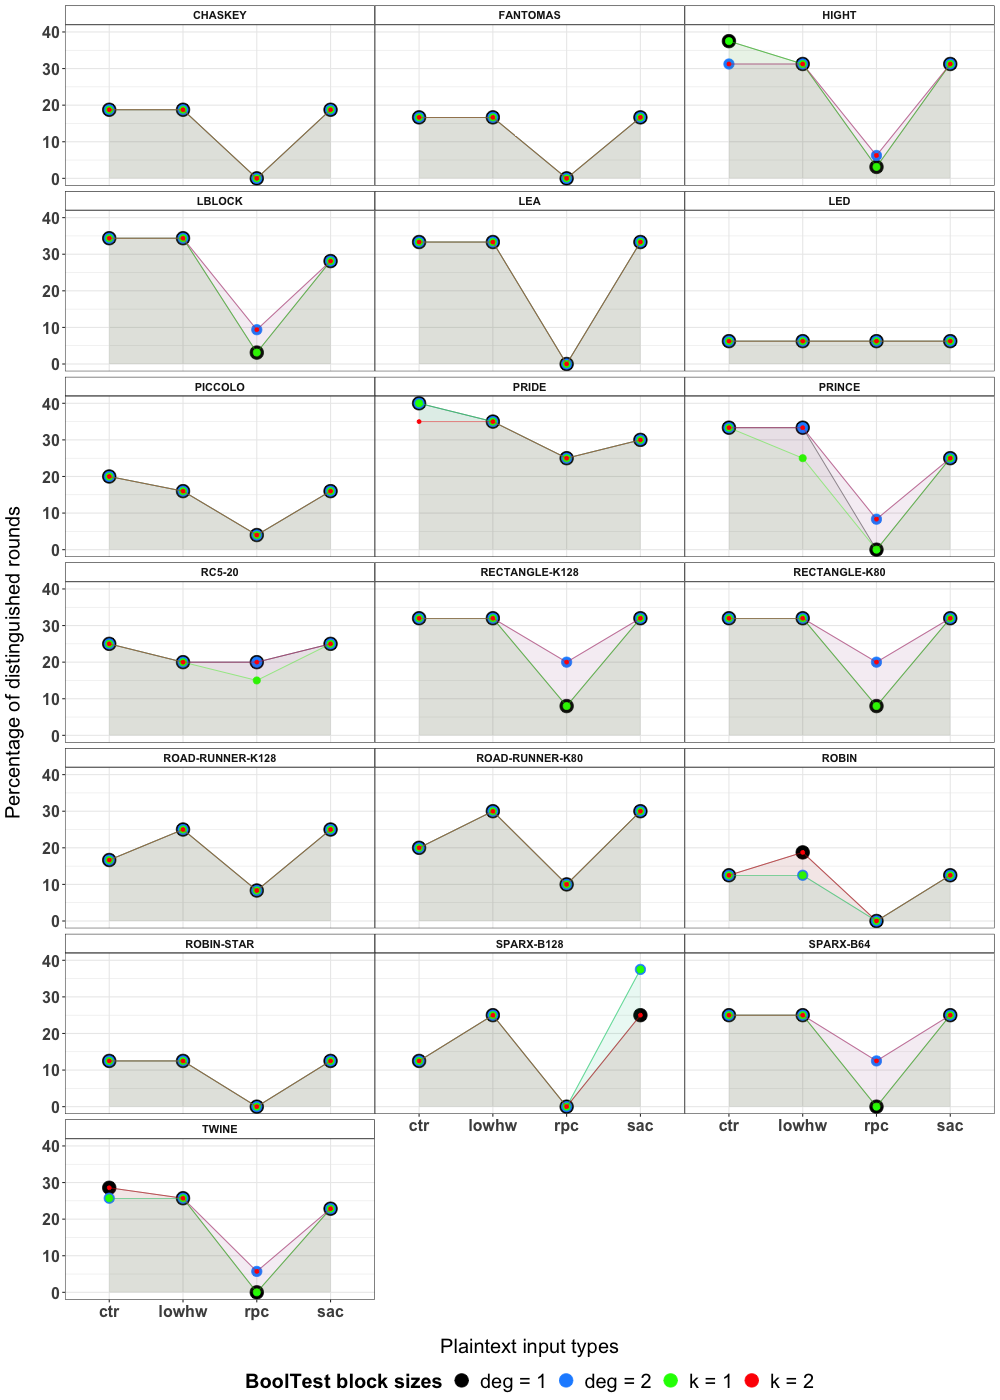
\includegraphics[width=\textwidth]{./images/pictures/bool_test_other_comparison.png}
	\caption{Comparison of results with respect to configuration of \textit{deg} and \textit{k} for BoolTest. Y-axis shows percentage of distinguished rounds for testing scenario denoted by x-axis. Each colored point represents highest rounds which was distinguished by BoolTest with corresponding parameter \textit{deg}, \textit{k} respectively.}
	\label{fig:bool_test_other}
\end{figure}

There are two ways of looking at \cref{fig:bool_test_other}. Either you can compare separately results for \textit{deg} (black and blue points) and \textit{k} (green and red), or you can see also comparison of combinations of results. For example, black and green point together, with blue and red under those two points, means the highest configuration was \textit{deg} = 1 and \textit{k} = 1. For full results for each combination of \textit{deg} and \textit{k} see \cref{fig:bool_test_other_comb}. Notice, that you can also combine together results from \cref{fig:bool_test_other} and \cref{fig:bool_test_block}, to find out full configuration. For example, for function SPARX-B128, you can see that highest result was achieved by configuration where block size is 512, \textit{deg} and also \textit{k} is 2.

From results for sequence types, it looks like that it is reasonable to increase \textit{deg} and \textit{k} parameters. As you can see in \cref{fig:bool_test_other}, at top of each sequence type, there is a blue or red point, this means that for all those results at least one of \textit{deg} and \textit{k} parameters were set to 2. The only difference is function HIGHT with counter plaintext type which is the only case, in which both 1 (\textit{deg} = 1, \textit{k} = 1) configuration resulted with exclusively highest round. However, this combination were not able to distinguish \textit{sac} and \textit{rpc} scenario for any function and round, even though other configurations were able to distinguish some of those sequences with significantly high Z-score. The best for \textit{rpc} scenario was combination with \textit{deg} = 2 and \textit{k} = 2.

\section{Results for pure PRNGs}
\label{sec:results for PRNGs}

In this section, we show the results of the statistical testing of 6 pure PRNGs with five testing scenarios. In four testing scenarios we used different seed source (ctr -- counter \textit{stream}, low hw -- low Hamming weight \textit{stream}, sac -- strict avalanche criterion and random stream) and in the last scenario (rpc -- plaintext/ciphertext \textit{stream}) we put together seed and some number of outputs from PRNG in resulting sequence. We conducted four experiments for each testing scenario; each has different reseed frequency (how many iterations of PRNG was executed before it was reseeded). We were reseeding after 10/100/1000 iterations or never (one seed for whole output sequence). For plaintext/ciphertext strategy we did not use never reseeding as it would be almost the same output as with random seed with never strategy (with the seed in the beginning), instead of never we added new frequency: 1 (a seed and first value is stored). 

Sequences were analyzed with the same tools as block ciphers — each sequence of size 8GB. In \cref{table:prng-results} there are two marks: \xmark~in a red cell which corresponds to resulting sequence was distinguished from a random stream and \cmark~in a green cell which means the sequence seems random from a statistical point of view. The number in brackets denotes how many tools were able to distinguish corresponding sequences. An asterisk in cell stands for notification that corresponding sequence was reseeded after each iteration instead of never reseeding (this was used for plaintext/ciphertext method for all functions).

As you can see in \cref{table:prng-results}, 4 out of 6 PRNGs were not able to produce a sequence which would be indistinguishable from a random stream in any combination of reseeding frequency and seed type. Only Xorshift and Mersenne Twister were able to produce such sequences. Xorshift produced such output with plaintext/ciphertext scenario. However, this might be caused by the size of the seed for Xorshift which is 32 bytes long, and the size of the output, which is only 4 bytes long. It means that if the reseeding frequency is 1 (new seed for every iteration), 88\% of the resulting sequence will be output from the random generator.

Mersenne Twister was able to produce the most sequences (out of six tested PRNGs) which were indistinguishable from a random sequence. From results, it seems that this PRNG produce biased sequences especially when it is reseeded often. See column with reseeding frequency 10 in  \cref{table:prng-results}, where all sequences were distinguished and also rpc strategy where PRNG is reseeded after each output. All those sequences were distinguished only by TestU01, mostly with Crush or Rabbit battery. It seems like Mersenne Twister is producing some bias which tests within those two batteries can identify.

\begin{table}[H]
	\centering
	\begin{tabular}{|c|c|c|c|c|c|}
		\hline
		\multirow{2}{*}{\textbf{\large Function}} & \multirow{2}{*}{\textbf{\large Testing method}} & 
		\multicolumn{4}{c|}{\textbf{\large Reseed frequency}} \\ \cline{3-6}
		& & Never / 1* & 10 & 100 & 1000 \\ \hline \hline
		
		\multirow{5}{*}{TestU01 - LCG} & counter &  \fd \xmark (4/4) & \fd \xmark (4/4) & \fd \xmark (4/4) & \fd \xmark (4/4) \\ \cline{2-6}
		& low hw &  \fd \xmark (4/4) & \fd \xmark (4/4) & \fd \xmark (4/4) & \fd \xmark (4/4) \\ \cline{2-6}
		& sac &  \fd \xmark (4/4) & \fd \xmark (4/4) & \fd \xmark (4/4) & \fd \xmark (4/4) \\ \cline{2-6}
		& rpc &  *\fd \xmark (4/4) & \fd \xmark (4/4) & \fd \xmark (4/4) & \fd \xmark (4/4) \\ \cline{2-6}
		& random &  \fd \xmark (4/4) & \fd \xmark (4/4) & \fd \xmark (4/4) & \fd \xmark (4/4) \\
		\hline \hline
		
		\multirow{5}{*}{TestU01 - MRG} & counter &  \fd \xmark (4/4) & \fd \xmark (4/4) & \fd \xmark (4/4) & \fd \xmark (4/4) \\ \cline{2-6}
		& low hw &  \fd \xmark (4/4) & \fd \xmark (4/4) & \fd \xmark (4/4) & \fd \xmark (4/4) \\ \cline{2-6}
		& sac &  \fd \xmark (4/4) & \fd \xmark (4/4) & \fd \xmark (4/4) & \fd \xmark (4/4) \\ \cline{2-6}
		& rpc &  *\fd \xmark (4/4) & \fd \xmark (4/4) & \fd \xmark (4/4) & \fd \xmark (4/4) \\ \cline{2-6}
		& random &  \fd \xmark (4/4) & \fd \xmark (4/4) & \fd \xmark (4/4) & \fd \xmark (4/4) \\
		\hline \hline
		
		\multirow{5}{*}{TestU01 - Xorshift} & counter &  \fd \xmark (1/4) & \fd \xmark (4/4) & \fd \xmark (4/4) & \fd \xmark (4/4) \\ \cline{2-6}
		& low hw &  \fd \xmark (1/4) & \fd \xmark (4/4) & \fd \xmark (4/4) & \fd \xmark (4/4) \\ \cline{2-6}
		& sac &  \fd \xmark (1/4) & \fd \xmark (4/4) & \fd \xmark (3/4) & \fd \xmark (2/4) \\ \cline{2-6}
		& rpc &  *\fn \cmark (0/4) & \fn \cmark (0/4) & \fd \xmark (1/4) & \fd \xmark (1/4) \\ \cline{2-6}
		& random &  \fd \xmark (1/4) & \fd \xmark (1/4) & \fd \xmark (1/4) & \fd \xmark (1/4) \\
		\hline \hline
		
		\multirow{4}{*}{STD - LCG} & counter &  \fd \xmark (4/4) & \fd \xmark (4/4) & \fd \xmark (4/4) & \fd \xmark (4/4) \\ \cline{2-6}
		& low hw &  \fd \xmark (4/4) & \fd \xmark (4/4) & \fd \xmark (4/4) & \fd \xmark (4/4) \\ \cline{2-6}
		& sac &  \fd \xmark (4/4) & \fd \xmark (4/4) & \fd \xmark (4/4) & \fd \xmark (4/4) \\ \cline{2-6}
		& rpc &  *\fd \xmark (4/4) & \fd \xmark (4/4) & \fd \xmark (4/4) & \fd \xmark (4/4) \\ \cline{2-6}
		& random &  \fd \xmark (4/4) & \fd \xmark (4/4) & \fd \xmark (4/4) & \fd \xmark (4/4) \\
		\hline \hline
		
		\multirow{5}{*}{STD - SWC} & counter &  \fd \xmark (4/4) & \fd \xmark (4/4) & \fd \xmark (4/4) & \fd \xmark (4/4) \\ \cline{2-6}
		& low hw &  \fd \xmark (4/4) & \fd \xmark (4/4) & \fd \xmark (4/4) & \fd \xmark (4/4) \\ \cline{2-6}
		& sac &  \fd \xmark (4/4) & \fd \xmark (4/4) & \fd \xmark (4/4) & \fd \xmark (4/4) \\ \cline{2-6}
		& rpc &  \fd \xmark (4/4) & \fd \xmark (4/4) & \fd \xmark (4/4) & \fd \xmark (4/4) \\ \cline{2-6}
		& random &  \fd \xmark (4/4) & \fd \xmark (4/4) & \fd \xmark (4/4) & \fd \xmark (4/4) \\
		\hline \hline
		
		\multirow{5}{*}{STD - Mersenne Twister} & counter &  \fn \cmark (0/4) & \fd \xmark (1/4) & \fn \cmark (0/4) & \fn \cmark (0/4) \\ \cline{2-6}
		& low hw &  \fn \cmark (0/4) & \fd \xmark (1/4) & \fn \cmark (0/4) & \fn \cmark (0/4) \\ \cline{2-6}
		& sac &  \fn \cmark (0/4) & \fd \xmark (1/4) & \fd \xmark (1/4) & \fd \xmark (1/4) \\ \cline{2-6}
		& rpc &  *\fd \xmark (1/4) & \fd \xmark (1/4) & \fd \xmark (1/4) & \fd \xmark (1/4) \\ \cline{2-6}
		& random &  \fn \cmark (0/4) & \fd \xmark (1/4) & \fd \xmark (1/4) & \fd \xmark (1/4) \\
		\hline
	\end{tabular}
	
	\caption{List of all results for PRNGs. Reseeding frequency correspond to number of iteration of PRNG before using new seed. \xmark~shows that the sequence was distinguished at least by one tool and \cmark~that the sequence seemed random for all tools.}
	\label{table:prng-results}
\end{table}

\chapter{Conclusion}
\label{chap:conclusion}

This thesis described and partly also practically presented stages of creating and testing of pseudo-random number generators (PRNGs). We theoretically presented several ways of construction of PRNGs. Then we explained the requirements put on PRNGs. We also described two ways of testing, whether those requirements are fulfilled. One of them is Linear and Differential cryptanalysis and the second is randomness testing.

We successfully extended CryptoStreams tool with 19 new lightweight block ciphers and six pure PRNGs including a new interface for this type of primitives. We also introduced a new test suite for implementation correctness for this tool to test chosen primitives with test vectors. All functions which were added within this thesis passed those tests. In practical part, we analyzed all functions added to CryptoStreams with four tools for randomness testing (NIST STS, Dieharder, TestU01, and BoolTest). 

During our analysis, we investigated the randomness properties of 1680 various sequences. Our analysis with BoolTest took more than 870 CPU days. We were not able to distinguish a full number of rounds for any block cipher, and we observed an acceptable security margin for each of them. The smallest value 60\% was obtained for function PRIDE  (we were able to distinguish 8 rounds out of 20). For tested pure PRNGs, it turned out that only Mersenne Twister and Xorshift can produce an output which is indistinguishable from a random sequence. However, it is probably caused by the fact, that none of those PRNGs is a cryptographically secure generator. This means that it is recommended not to use those generators within cryptographic applications.

We also showed a comparison of the success of statistical tools in distinguishing between analyzed data and truly random sequences. Concerning statistical batteries, in general, TestU01 software tool achieved better results than older batteries NIST STS and Dieharder. However, for lightweight block ciphers, BoolTest tool produced comparable, in some cases even slightly better, results than batteries from TestU01. Regarding pure PRNGs, TestU01 was mostly able to distinguish their output. TestU01 was the only tool, which was able to distinguish sequences produced by Mersenne Twister.

When comparing batteries within TestU01 (Alphabit, Block Alphabit, Crush, Rabbit and Small Crush) the highest results for block ciphers were achieved mostly by Block Alphabit and Crush. However, for pure PRNGs (Mersenne Twister and Xorshift), we observed worse results than for block ciphers for Block Alphabit battery. Those sequences were mostly distinguished by batteries Crush and Rabbit.

\section{Future work}

TestU01 software tool provides a large number of implementations of PRNGs. We have not incorporated all of them within CryptoStreams because we were not able to find parameters for each PRNG. Also, for some parameters they produce 8 bytes long number which has upper bits filled with zeros only, which may cause problems when testing randomness, more information in \cref{subsec:pure-generators}. However, we provided an interface in CryptoStreams, so after resolving those issues for each PRNG it should be easy to incorporate them and conduct an analysis similar to one provided in this thesis.

Other interesting results could be obtained by expanding the number of tested parameters, especially for BoolTest. We concluded that it is reasonable to increase values of BoolTest parameters \textit{deg} and \textit{k} because configurations with at least one of \textit{deg} and \textit{k} set to 2 almost always distinguished same or higher number of rounds. We did not include a value 3 for those parameters because it was unfeasible for us with the combination of other computations. However, when doing only this experiment, it would be still reasonably feasible, and the results could disprove or provide more certainty to our conclusion, whether it is reasonable to increase parameters \textit{deg} and \textit{k}.

While some tests in statistical batteries require a significant amount of data (for example Big Crush battery in TestU01 needs more than 60GB of data), BoolTest is built so that it can work with several MB of data, with comparable results to batteries. We tested all tests with 8GB so that we can compare the performance of tools under equal conditions. However, another interesting extension would be an analysis of the effect of decreasing size of analyzed data on results of BoolTest.


%%bibliography

\setcounter{biburllcpenalty}{7000}
\setcounter{biburlucpenalty}{8000}
\printbibliography[heading=bibintoc] %% Print the bibliography.

\appendix{}

\chapter{Data attachment}

The data attachment available in the thesis repository\footnote{\url{http://is.muni.cz/th/422190/fi_m/}}, which contains source codes of tools we extended or modified and all obtained results including configuration files.

\begin{itemize}
	\item \texttt{CryptoStreams}
	
	Source code of CryptoStreams. The corresponding repository commit is \texttt{1031817}.
	
	\item \texttt{CryptoStreams.wiki}
	
	Documentation of CryptoStreams with added materials about PRNGs. Corresponding repository commit is \texttt{82047ff} from 2018-08-13.
	
	
	
	\item \texttt{results}
	
	All collected results from thesis experiments. It contains BoolTest raw results, where each file contains also a configuration, including a configuration for CryptoStreams. There are also our own scripts which merge results from BoolTest and batteries and produce all comparisons presented in this thesis, including \texttt{CSV} files used by scripts for generation graphs. Folder with batteries contains scripts for cooperation of CryptoStreams with RTT.
	
	
	\item \texttt{thesis-src}
	
	Thesis text source including bibliography and used images.
\end{itemize}

\chapter{Additional comparisons for BoolTest results}

\begin{figure}[htp]
	\centering
	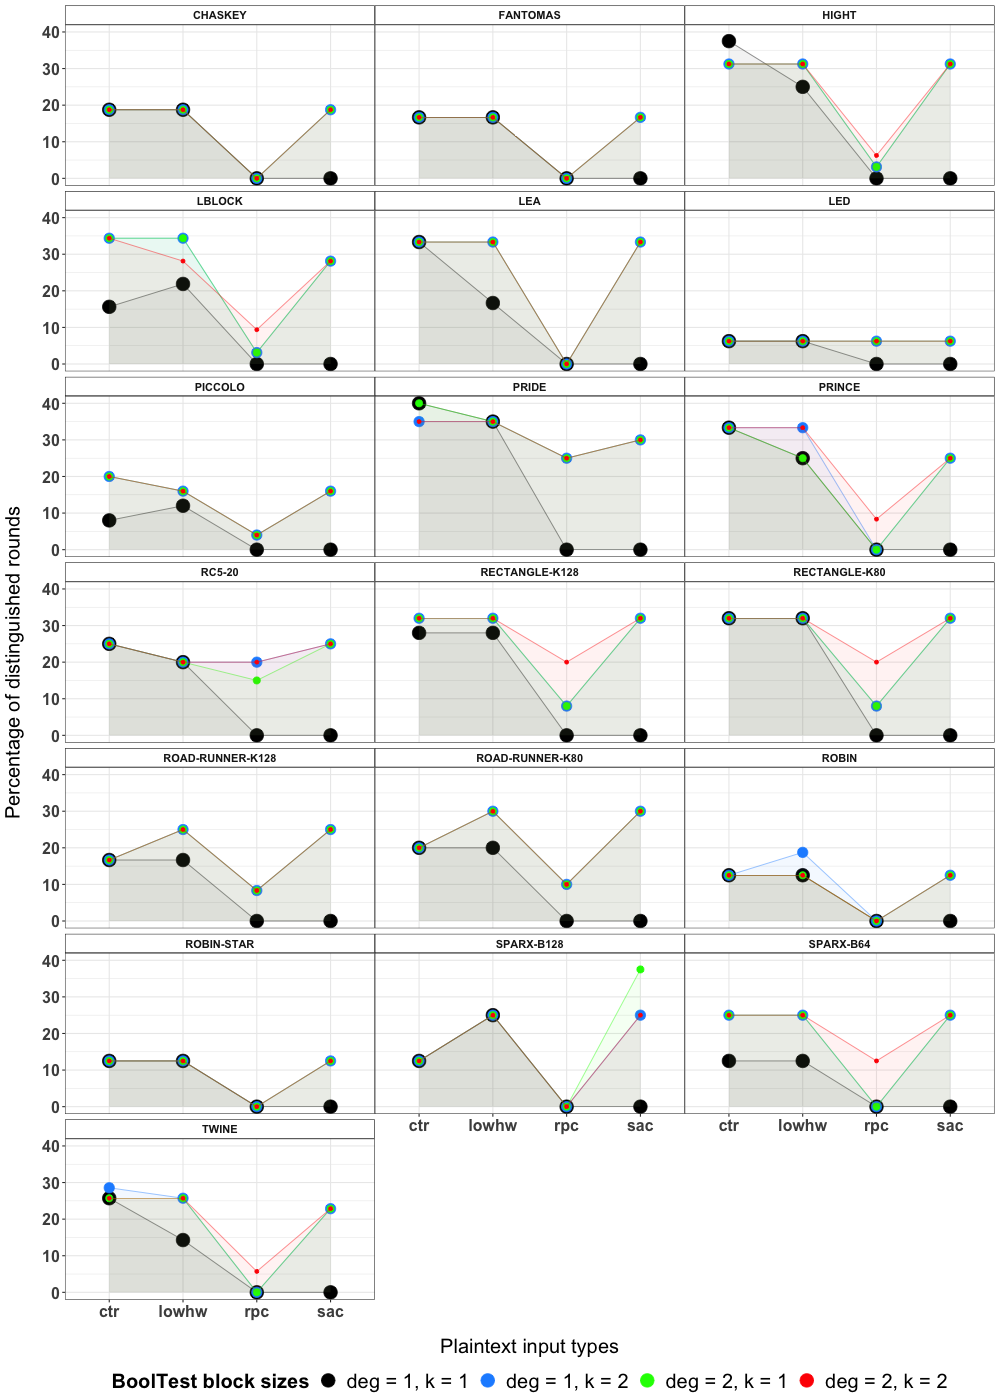
\includegraphics[width=\textwidth]{./images/pictures/bool_test_other_comparison_combinations.png}
	\caption{Comparison of results with respect to configuration of combination of \textit{deg} and \textit{k} for BoolTest. Y-axis shows percentage of distinguished rounds for testing scenario denoted by x-axis. Each colored point represents highest rounds which was distinguished by BoolTest with corresponding parameters \textit{deg}, \textit{k} respectively.}
	\label{fig:bool_test_other_comb}
\end{figure}

\end{document}
